\documentclass[fleqn,usenatbib]{mnras}
\usepackage{graphicx} % Required for inserting images
\usepackage{amsmath}      % Advanced math formatting
\usepackage{amssymb}      % Symbols like \mathbb
\usepackage{multicol}        % Multi-column entries in tables
\usepackage{bm}		% Bold maths symbols, including upright Greek
\usepackage{pdflscape}	% Landscape pages
\usepackage{wasysym}    % Astronomy Symbols
\usepackage{upgreek}    % Upright Greek Symbols
%\usepackage{gensymb}    % General Symbols
\usepackage{orcidlink}  % orcid
\usepackage[table]{xcolor}
\usepackage[normalem]{ulem}


\interfootnotelinepenalty=10000
% Use vector fonts, so it zooms properly in on-screen viewing software
% Don't change these lines unless you know what you are doing
\usepackage[T1]{fontenc}
\usepackage{ae,aecompl}
\usepackage{newtxtext,newtxmath} % MNRAS-approved fonts

\newcommand{\bibtex}{\textsc{Bib}\!\TeX}
\newcommand{\orcid}[1]{\href{https://orcid.orffi#1}{\textcolor[HTML]{A6CE39}{\aiOrcid}}}
\renewcommand{\figureautorefname}{Fig.}
\renewcommand{\equationautorefname}{equation}
\renewcommand{\sectionautorefname}{Section}
\renewcommand{\subsectionautorefname}{Section}
\renewcommand{\subsubsectionautorefname}{Section}
\newcommand{\mss}[1]{\textbf{\textcolor{purple}{[MSS: #1]}}}
\newcommand{\sod}[1]{\textbf{\textcolor{green}{[SOD: #1]}}}


%%%%%%%%%%%%%%%%%%%%%%%%%%%%%%%%%%%%%%%%%%%%%%%%%%%%%%%%%%%%
\begin{document}

\author[S. DeLaurentiis et al.]{
Stanislav DeLaurentiis$^{1,2}$\orcidlink{0000-0002-8922-825X}\thanks{Contact e-mail: \href{mailto:sod2112@columbia.edu}{sod2112@columbia.edu}}, Zoltan Haiman$^{2}$\orcidlink{0000-0003-3633-5403}\thanks{Contact e-mail: \href{mailto:zh2007@columbia.edu}{zh2007@columbia.edu}}, Magdalena Siwek$^{2}$\orcidlink{0000-0002-1530-9778}\thanks{Contact e-mail: \href{mailto:mss2334@columbia.edu}{mss2334@columbia.edu}}, Roman Rafikov$^{1,3}$\orcidlink{0000-0002-0012-1609}\thanks{Contact e-mail: \href{mailto:rrr34@cam.ac.uk}{rrr34@cam.ac.uk}} \\
\\
% List of institutions
$^{1}$Department of Astronomy, Columbia University, 550 W. 120th Street, New York, NY 10027, USA\\
$^{2}$Department of Applied Mathematics and Theoretical Physics, University of Cambridge, Wilberforce Road, Cambridge CB3 0WA, UK\\
$^{3}$Institute for Advanced Study, Einstein Drive, Princeton, NJ 08540, USA
}


\title{Preferential Accretion onto Eccentric and Unequal Binary Black Hole Systems}


% These dates will be filled out by the publisher
\date{}

% Enter the current year, for the copyright statements etc.
\pubyear{2024}

% Don't change these lines
\label{firstpage}
\pagerange{\pageref{firstpage}--\pageref{lastpage}}
\maketitle
%%

\begin{abstract}
    Supermassive Binary Black Holes (SMBBHs) are expected to be surrounded by Circumbinary Disks (CBDs) which affect the binary through gravitational torques and accretion. It has been reported that the binary can experience ``preferential accretion'' where one black hole (BH) out-accretes the other for hundreds of orbits, but the phenomenon has yet to be fully described or understood.  In this work, we utilize a suite of 80 SMBBH hydrodynamic simulations with varying mass ratios ($q_b$) and eccentricity ($e_b$) in order to robustly delineate the behavior of preferential accretion, determine its relationship to the structure of the CBD, and study its observational consequences. In this paper we report the most extensive series of measurements for $\dot{q}$, the rate of change of the binary mass-ratio, and $\lambda(t)$ the ratio of the BH accretion rates. We also share our findings that a) the accretion behavior onto one BH over the other is strongly tied to the precession of the CBD, b) there can be sub and super-eddington accretion in a single binary, and c) there exists a regime where the CBD can drive the binary away from $q_b =1 $. Given these findings, we suggest flickering jets and an under-density of LISA events $q_b=1$ as potential observable consequences.
\end{abstract}

\section{Introduction}

Cosmic structure forms hierarchically and galaxy mergers are expected to result in gravitationally bound Super-Massive Binary Black Holes (SMBBHs) \citep{white_rees_78,begelman_blandford_rees_80}. During galactic merger, it is also expected that the inter-stellar medium from the proto-galaxies are funneled to the galactic center. This creates a reservoir of material that, due to the conservation of angular momentum and the binary's gravitational potential, forms a circumbinary disk (CBD). Many aspects of the CBD have been well studied in the literature, in both the SMBBH and the star-planet contexts. It has been shown that the binary can influence the CBD, creating eccentric structure and precessing eigenmodes, \citep{lubow_91, whitehurst_94, nelson_2003, Goodchild_2006, paardekooper_2008, kley_2008, shi_2012, miranda_munoz_lai_2017, Thun_2017,munoz_lithwick_2020, Lubow_2022, siwek_prefacc} and that the CBD can in turn influence the binary---changing both its semi-major axis and eccentricity \citep{Tiede_2020, zrake_2021, dorazio_2013, siwek_cbdorbevol, dorazio_duffel, farris_2014}, as well as exciting precession of the binary itself \citep{tiede_24_diskinducedprecession, dittmann_prec, calcino_prec}. However, crucially, the binary also accretes from the circumbinary disk, influencing both the mass-ratio and associated light-curves of the system (e.g \citet{siwek_prefacc, ryan_2022}). 



It has been a widely known result of CBD studies that the accretion on to the binary ($\dot{M}_{\rm{b}} = \dot{M}_1 + \dot{M}_2$) is not steady but experiences variability through time. Near equal-mass ratio ($q_b>0.7$) circular binaries display a sawtooth pattern with a period of about $5$ binary orbital periods ($\tau_{\rm{b}}$) potentially due to the presence of an $\rm{m}=1$ over-density traveling at the inner edge of the CBD \citep{MacFadyen_08, miranda_munoz_lai_2017, munoz_miranda_lai_19,ryan_2022}. Eccentric and unequal mass-ratio binaries too display variability on the order of a binary period \citep{miranda_munoz_lai_2017, munoz_miranda_lai_19, ryan_2022}.In order to study how the binary, as an entity, accreted material from the circumbinary disk, \citet{Tiede_22} tracked the paths of passive tracer particles in a two-dimensional grid-based hydrodynamical codes. They determined that much of the gas is viscously transported from the outer disk before adopting a ballistic trajectory and ultimately accreting on to the BHs near the inner edge. They also delineate an ``accretion horizon'' of $1.01$ the semi-major axis of the binary ($a_b$), a radius that past which any material enters is accreted.

However, studies have also pointed out the discrepancy between the accretion behaviors of the primary and secondary components of the SMBBH  (e.g  \citet{miranda_munoz_lai_2017, siwek_prefacc, Dorazio_24_pref_mention}). Namely, the secondary tends to accrete, on average, at a greater rate than the primary in what has become known as ``preferential accretion''---pushing the system to equal mass ratio ($q_b=1$) \citep{miranda_munoz_lai_2017, siwek_prefacc}. While systems with $q_b = 1$ generally accrete at equal rates, suggesting a stable equilibrium at $q_b = 1$, studies have reported that at certain eccentricities (e.g., $e_b = 0.5$ and $e_b = 0.6$), the binary can undergo transient "symmetry breaking." (see Figure 7 in \citet{munoz_miranda_lai_19}). In these instances, one black hole temporarily accretes more than its counterpart before its accretion rate is suppressed, while the other experiences an enhanced accretion rate.
 

This process was explored in \citet{siwek_prefacc} by studying the accretion rate behavior across $50$ 2D hydrodynamic simulations of SMBBHs in CBDs, sampling different binary parameters $q_b$ and $e_b$. \citet{siwek_prefacc} reported time averaged values of $\lambda = \dot{M}_2/\dot{M}_1$, the ratio of the secondary's accretion rate to the primary's, for their simulation suite and displayed snapshots of the corresponding CBD. \citet{siwek_prefacc} report that low-eccentricity binaries display larger values of $\lambda$ than high-eccentricity binaries ($e_b > 0.6$). Further, the process of the flip in preferential accretion was suggested to be associated with the behavior of the CBD. Namely, it was associated with a unique disk behavior they called ``forced precession''. \citet{DeLaurentiis24} also discussed the preferential accretion rate of the binary, suggesting it be understood in geometric terms though the distance from the BHs to the CBD. 

The protoplanetary disk community have run two and three dimensional smoothed particle hydrodynamic (SPH) simulations of CBDs in interest of understanding the accretion onto the primary and secondary \citep{Gunther_Kley_02,Ochi_05, Young_15}. In simulations run for for $\leq 100 \tau_{\rm{b}}$ they found that the primary can out-accrete the secondary due to streamlines that, despite entering the Lagrange point L2, have such high angular momentum that they are able to flow to the counterpart \citep{Ochi_05, Young_15}. Similar findings were suggested in \citet{Tiede_22}.

Despite these efforts we are still yet to fully characterize and understand the rich detail of accretion onto the individual components of a binary in a CBD system. Thus, in the following work we build on \citet{siwek_prefacc} and, with the consent of the authors, use the larger simulation suite of \citet{siwek_cbdorbevol} to report the largest binary parameter sweep study on ``preferential accretion''. Further, we more robustly characterize the accretion behavior by applying unique numerical techniques and more fine-grained analytic tools. 

In \autoref{sec:methods} we briefly discuss the technical details of the simulations, the key concepts from linear theory we draw upon, and the key techniques we employ. In \autoref{sec:results} we present our findings: detailing the temporal behavior of preferential accretion and mass-ratio evolution and describe how that varies with initial binary $q_b$ and $e_b$. In \autoref{sec:observations} we detail the consequences our findings have on observations. We discuss how our results could suggest  a) jets that periodically switch on and off, ``flickering'', and a population of SMBBHs with $q_b \neq 1$. In \autoref{sec:conclusion} we summarize our key findings and discuss next steps.


\section{Analytic Tools and Numerical Methods}\label{sec:methods}
In the following section we briefly describe the setup of the \citet{siwek_prefacc, siwek_cbdorbevol} simulations, the concepts from linear disk theory we employed, and the numerical tools we leveraged.
\subsection{Simulation Setup}
In the following we briefly describe the setup for the simulations of interest, but please see \citet{siwek_prefacc,siwek_cbdorbevol} for a more thorough discussion.



\citet{siwek_prefacc, siwek_cbdorbevol} performed 2D hydrodynamical simulations of binary black holes embedded in a finite, locally isothermal disk with an $\alpha$-viscosity of $\alpha=0.1$ and an aspect ratio of $h=0.1$. The disk is initialized according to a power law function that places the inner edge of the cavity at $2a_b$ and the outer edge at $\approx 50a_b $. The binary-disk system spans a computational grid of $300 a_b \times 300a_b$ with open boundary conditions, allowing the disk to viscously spread over time and reach a quasi-steady state. 

The binary is modeled as two sink particles with a mass-ratio $q_b$ and radii $r_{\rm{s}} = 0.03 a_{\rm{b}}$, moving on a fixed Keplerian orbit of eccentricity $e_{\rm{b}}$. The fraction of gas accreted from each gas cell at each time step by the sink particle is $\gamma_0 \left( 1 - \frac{r_{ij}}{r_{\rm{s}}}\right)^2$ where $r_{ij}$ is the radial distance from the jth sink particle to the ith gas cell. In addition to the mass of the gas cell, the sink also accretes the gas' linear momentum.

The simulations, conducted with the moving-mesh code AREPO, used Voronoi tessellation to generate a grid of cells and explored a wide parameter space for $q_b$ and $e_b$ across the sets $q_b \in \{ 0.1, 0.2, 0.3, 0.4, 0.5, 0.6, 0.7, 0.8, 0.9, 1.0 \}$ and $e_b \in \{0.1, 0.2, 0.3, 0.4, 0.5, 0.6, 0.8 \}$. The simulations were run for $10,000$ orbits, with surface density snapshots recorded at aopocenter every $10$ orbits. Accretion rates, however, were recorded independently at a much higher cadence, with a time-step of $\approx 0.01$ orbits.



\subsection{Disk Theory}

In order to illuminate the relationship between the accretion of the binary and the behavior of the CBD we must first characterize the time-variable behavior and attributes of the disk. Namely, we focus on the eccentricity and precession of the disk. 

Gas eccentricity within CBDs is expected to grow through mechanisms such as eccentric Lindblad resonances (ELRs) or spiral shock pumping at the cavity edge \citep{lubow_91, whitehurst_94, paardekooper_2008, kley_2008, shi_2012}. While ELRs and spiral shocks promote eccentricity growth \citep{lubow_91, shi_2012}, viscous damping \citep{Goodchild_2006} and orbit crossings \citep{Statler_2001} act to suppress it. Previous 2D simulations have found steady-state eccentricity profiles, indicating that these competing effects can reach equilibrium \citep{miranda_munoz_lai_2017, siwek_prefacc}.Further, 2D and 3D hydrodynamical simulations have found significant eccentricity near the inner edge of the disk (the cavity), with eccentricity declining outward \citep{MacFadyen_08, miranda_munoz_lai_2017, siwek_prefacc, ragusa_lynch}. Similar trends have been seen in magneto-hydrodynamic simulations \citep{shi_2012}, suggesting that eccentricity is a robust characteristic of CBDs.

Additionally, simulations have demonstrated that the CBD can precess \citep{nelson_2003, shi_2012, miranda_munoz_lai_2017, Thun_2017, siwek_prefacc}, with precession frequencies often attributed to the eigenmodes of a Schrödinger-like equation for eccentricity evolution \citep{Goodchild_2006, shi_2012, Teyssandier_2016, Lee_2019, munoz_lithwick_2020, Lubow_2022}.


A robust study of the eccentricity and precession of both the bulk of the disk and the cavity in hydrodynamic simulations was conducted by \citet{DeLaurentiis25}. Utilizing the same suite of simulations as this paper, they delineate the shape of the non-linear inner edge of the circumbinary disk, the cavity, by extracting the dominant Fourier modes of the associated isodensity contour.


While alternative explanations have been proposed \citep{Artimowicz_83_og_polish}, it has widely been assumed that the preferential accretion of the binary is related to the relative closeness of the components to the CBD's inner edge \citep{Rafikov_16_accretion}. In order to test this dependence we utilize the results for the cavity shape and its precession period from \citet{DeLaurentiis25} in order to build a robust time-dependent geometric picture of the binary in the cavity.


\subsection{Numerical Techniques}
As discussed earlier, in order to highlight the link between accretion and the behavior of the CBD, we are interested in understanding both as time-dependent quantities. The shape of the CBD is inherently time-dependent due to its precession\footnote{While, the eccentricity and semi-major axis are strictly time-dependent, we find that for most systems the shape of the cavity seems to achieve a steady state and its time-dependence is due to its apsidal precession alone.}. Since our simulation runs output snapshots every $10$ orbits, the time-series associated with our CBD is constrained to a $10 \tau$ cadence.


The accretion rate is time-dependent too. For each sink, the simulation tracks the mass accreted $\Delta m$ at time-step $t$, with a maximum cadence of $0.01 \tau$. As we are interested in comparing the accretion rate to the behavior of the CBD, we down-sample the high cadence accretion rate data to yield a time-series that matches the $10$ orbit cadence of the CBD time-series. We do this by summing the instantaneous mass accreted over $10$ orbit non-overlapping sliding windows and dividing it by the window size of $10$ orbits. After we transform the accretion rates for each BH into the lower cadence of $10$ orbits via the aforementioned method, we construct our preferential accretion quantity $\lambda(t) = \frac{\dot{M}_2(t)}{\dot{M}_1(t)}$, the ratio of the accretion rate of the secondary to the primary.


%SOD:Turns out the below is wrong. I ran both to check, and I think what I was doing before was averaging over lambda, and applying sav-gol filter. Not really crucial to comment on then...
% Since our accretion rate data is not of uniform cadence, it is only appropriate to calculate accretion rates using this method. If we were to instead conduct sliding window averages over instantaneous accretion rates $\Delta\frac{ m_{i+1}}{t_{i+1} - t_i}$ as done in \citet{siwek_prefacc} we achieve time-dependent behaviors. This is exemplified in the following plot of a xx yy binary. Note how though both are of the same candence there is a factor of two difference between the ouputs. While this method is critical to our time-dependent accretion rates, this does not strongly affect the averaged values reported in figure 4 of \citet{siwek_prefacc}. 


We also report the rate of change of the mass-ratio $\dot{q}(t)$. We define it as 
\begin{equation}\label{eqn:q_dot}
    \dot{q} = \frac{(1+q_b(t))(\lambda(q_b) - q_b(t))}{1 + \lambda(q_b)}\frac{\dot{M}_1 +\dot{M}_2}{M_1 + M_2}
\end{equation}
where
\begin{equation}
    q(t) = \frac{M_2 (t)}{M_1 (t)}
\end{equation}
and the mass of each BH
\begin{equation}
    M_j(t) = \sum_{0}^{t} (M_j(t=0) + \Delta m(t))
\end{equation}
is simply the running sum. Again, we note that all time-variable inputs are first transformed to be of $10$ orbit cadence via the aforementioned procedure.


\section{Results}\label{sec:results}
In the following sections we report our key results. Namely, in \autoref{sec:pref_acc} we detail the behavior of $\lambda(t)$ and report its mean value and, if time variable, its period. In \autoref{sec:preliminary_analysis}, we make some preliminary investigation into the CBD's effect on the accretion behavior. In \autoref{sec:mass_ratio} we calculate the rate of change of the mass ratio, and highlight an instance of the binary accreting away from unity.

\subsection{Preferential Accretion}\label{sec:pref_acc}

\begin{figure*}
    \centering
    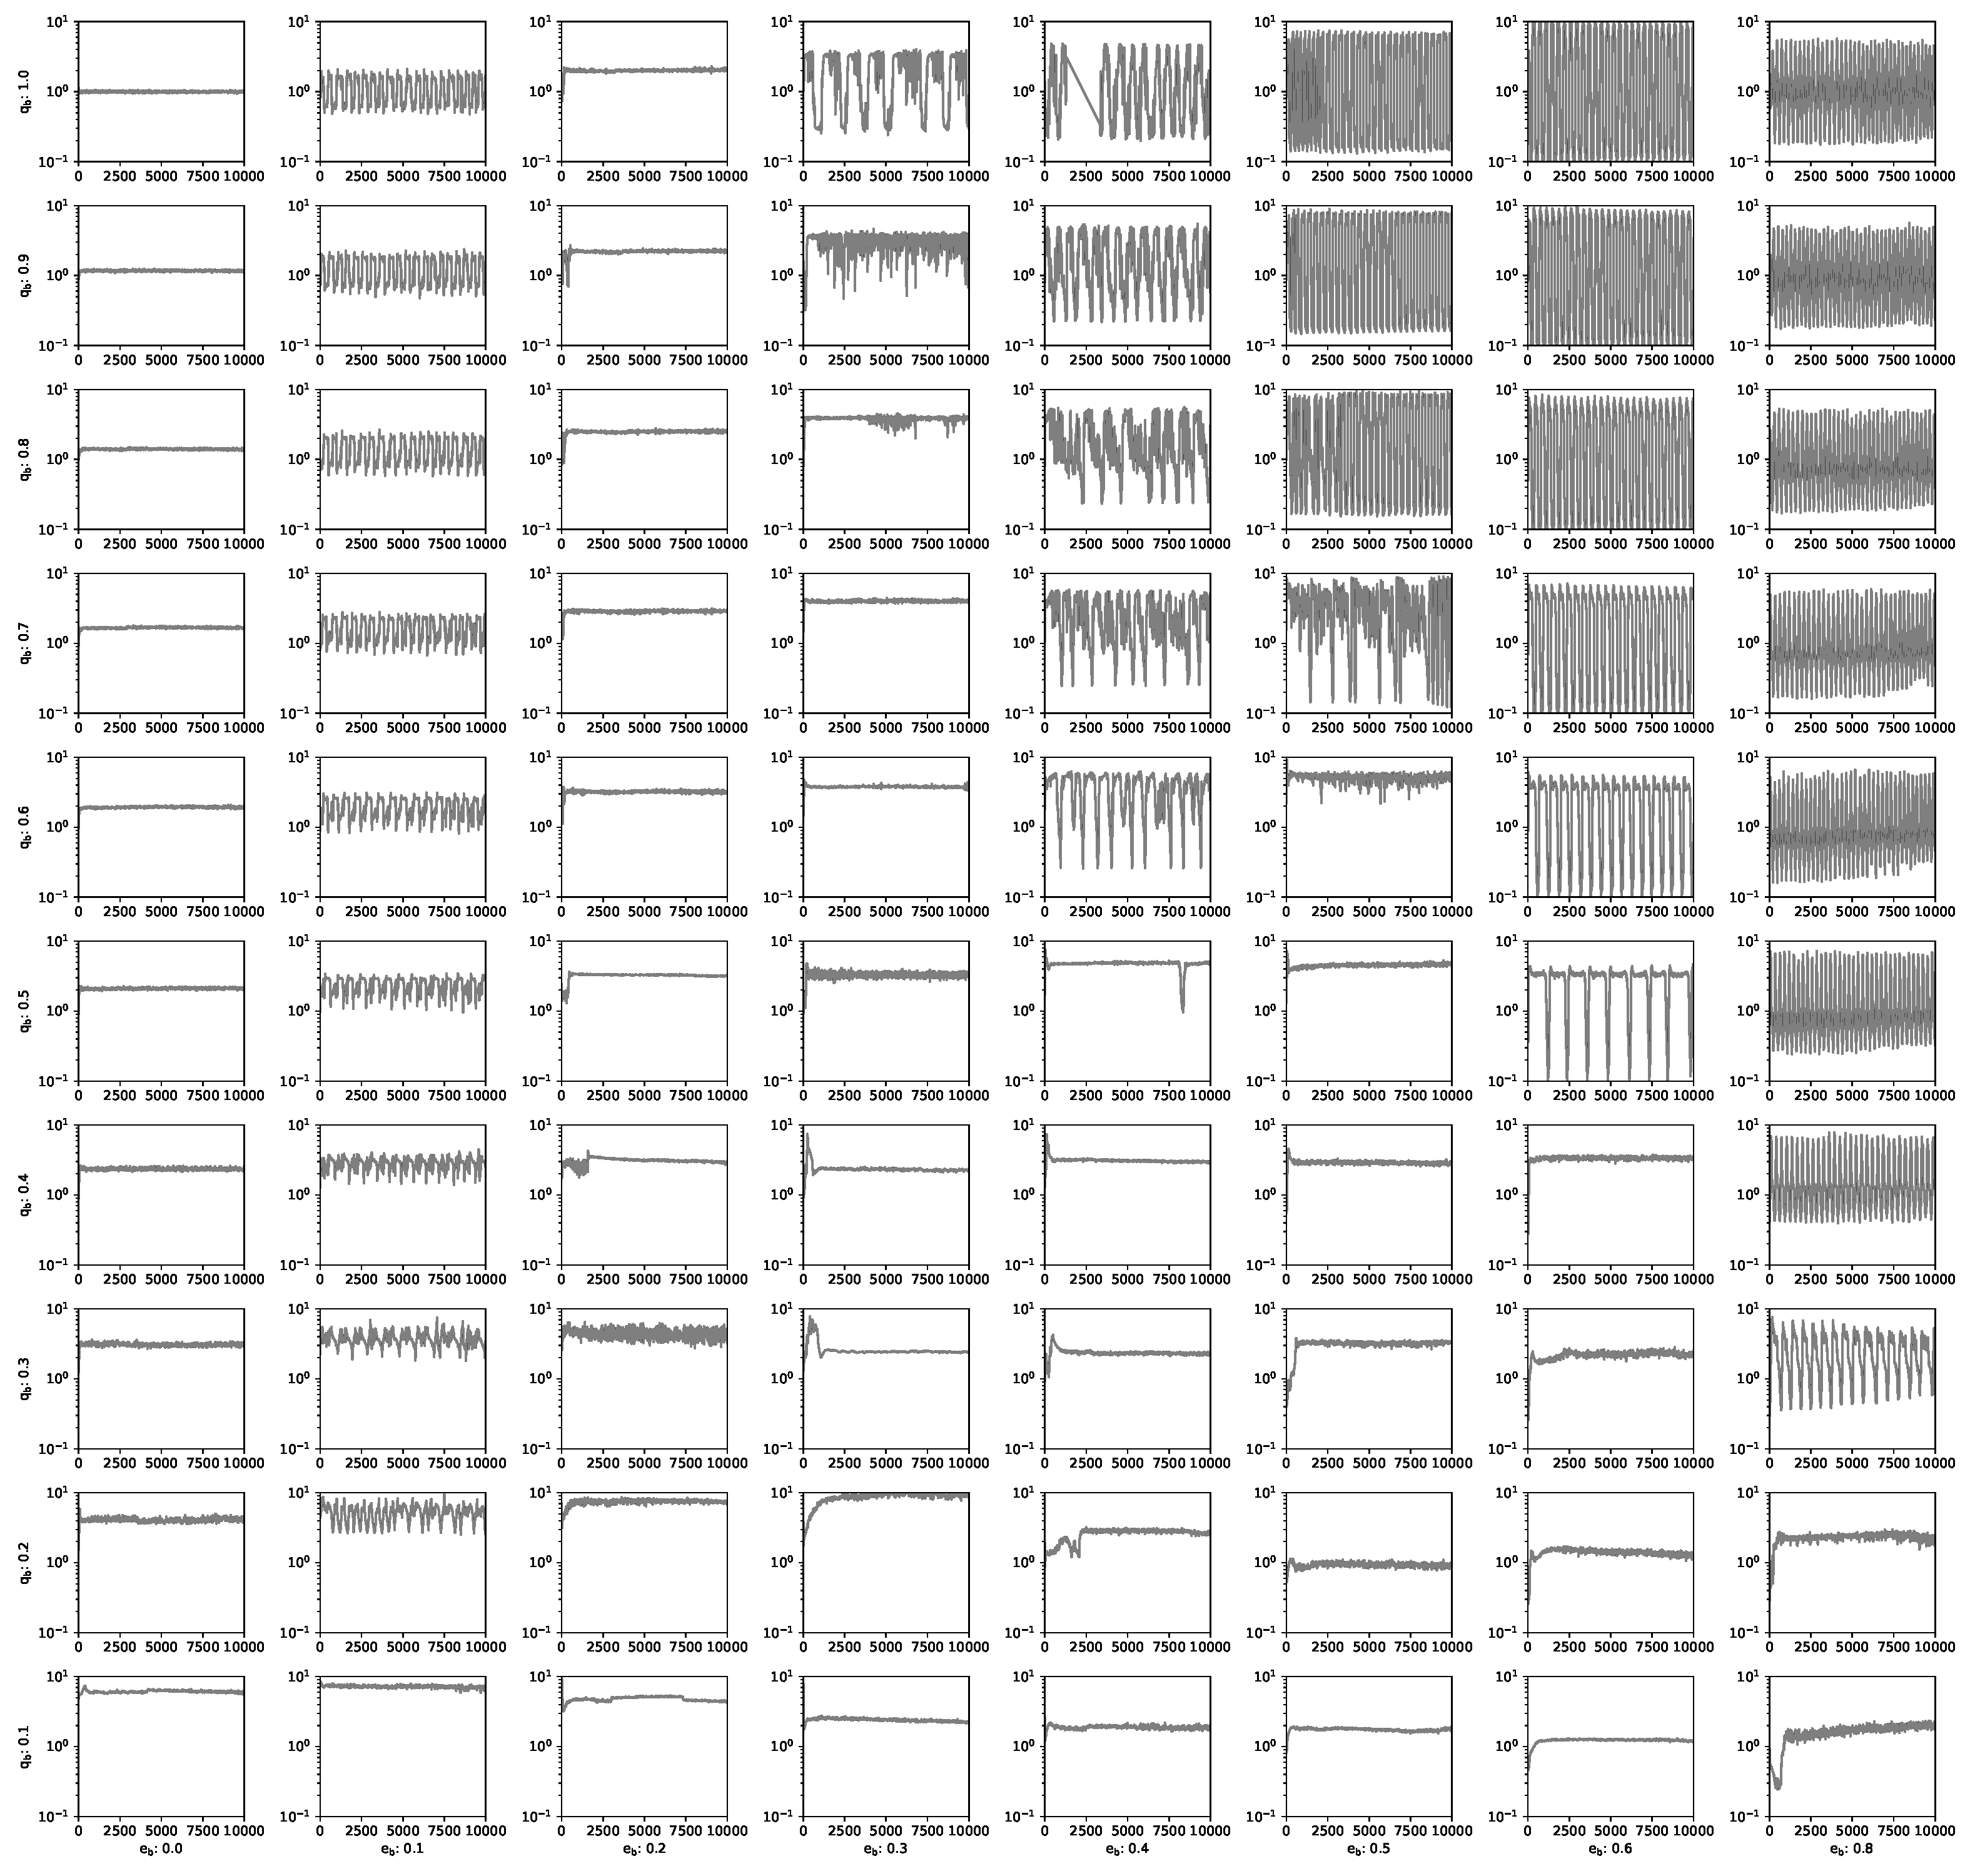
\includegraphics[width=1\textwidth]{lambda_fixed_magda_ratio_0_10000.pdf}
    \caption{$\lambda(t)$ for our binary simulation suite. Each panel represents a unique simulation, with $\lambda(t)$ on the y-axis and time on the x-axis. The panel's position on the larger grid signifies its binary parameters, with $e_b$ being constant along columns and increasing from left to right, and $q_b$ being constant along rows and increasing from bottom to top.}
    \label{fig:lambda_full}
\end{figure*}


In \autoref{fig:lambda_full} we plot our $\lambda(t)$ time-series for the entirety of our simulation suite. The figure is structured such that each panel represents a unique simulation. The rows represent simulations of the same mass-ratio $q_b$, whereas the columns represent simulations of the same eccentricity $e_b$. The left-most columns are the least eccentric binaries, and the upper-most rows are the most equal-mass binaries.

What first strikes us in \autoref{fig:lambda_full} is the broad division of $\lambda(t)$ into being time-stable or time-varying. Broadly, many low $e_b$, low $q_b$ binaries are time-stable. Though some experience a sharp change in behavior in the first $2000$ orbits associated with an expected initial instability \citet{moriwaki_04, DeLaurentiis25}, they soon reach a near-constant value. This time-stable behavior is well exemplified by the $e_b = 0.3$, $q_b = 0.3$ binary \footnote{Though some binaries (e.g $e_b = 0.$, $q_b = 0.3$) experience noticeable modulation around this constant value, the dichotomy between time-varying and time-stable $\lambda(t)$ values remain clear.}. Others, show time-variable behavior with oscillations in $\lambda(t)$ spanning two orders of magnitude, such as $e_b=0.6 , \, q_b=1.0$.

\renewcommand{\arraystretch}{1.5} % Adjust row height
\begin{table}
\centering
\begin{tabular}{|c|c|c|c|c|c|c|c|c|} 
    \hline
    \textbf{1.0} &
    \cellcolor{red}\textcolor{white}{S} & 
    \cellcolor{blue}\textcolor{white}{V} &
    \cellcolor{red}\textcolor{white}{S} &
    \cellcolor{blue}\textcolor{white}{V} & 
    \cellcolor{blue}\textcolor{white}{V} & 
    \cellcolor{blue}\textcolor{white}{V} & 
    \cellcolor{blue}\textcolor{white}{V} & 
    \cellcolor{blue}\textcolor{white}{V} \\ 
    \hline
    \textbf{0.9} & 
    \cellcolor{red}\textcolor{white}{S} & 
    \cellcolor{blue}\textcolor{white}{V} & 
    \cellcolor{red}\textcolor{white}{S} &
    \cellcolor{red}\textcolor{white}{S} & 
    \cellcolor{blue}\textcolor{white}{V} & 
    \cellcolor{blue}\textcolor{white}{V} & 
    \cellcolor{blue}\textcolor{white}{V} & 
    \cellcolor{blue}\textcolor{white}{V} \\ 
    \hline
    \textbf{0.8} & 
    \cellcolor{red}\textcolor{white}{S} & 
    \cellcolor{blue}\textcolor{white}{V} & 
    \cellcolor{red}\textcolor{white}{S} &
    \cellcolor{red}\textcolor{white}{S} & 
    \cellcolor{blue}\textcolor{white}{V} &
    \cellcolor{blue}\textcolor{white}{V} &
    \cellcolor{blue}\textcolor{white}{V} &
    \cellcolor{blue}\textcolor{white}{V} \\ 
    \hline
    \textbf{0.7} & 
    \cellcolor{red}\textcolor{white}{S} &
    \cellcolor{blue}\textcolor{white}{V} &
    \cellcolor{red}\textcolor{white}{S} & 
    \cellcolor{red}\textcolor{white}{S} & 
    \cellcolor{blue}\textcolor{white}{V} & 
    \cellcolor{blue}\textcolor{white}{V} & 
    \cellcolor{blue}\textcolor{white}{V} & 
    \cellcolor{blue}\textcolor{white}{V} \\ 
    \hline
    \textbf{0.6} & 
    \cellcolor{red}\textcolor{white}{S} & 
    \cellcolor{blue}\textcolor{white}{V} & 
    \cellcolor{red}\textcolor{white}{S} & 
    \cellcolor{red}\textcolor{white}{S} & 
    \cellcolor{blue}\textcolor{white}{V} & 
    \cellcolor{red}\textcolor{white}{S} & 
    \cellcolor{blue}\textcolor{white}{V} & 
    \cellcolor{blue}\textcolor{white}{V} \\ 
    \hline
    \textbf{0.5} & 
    \cellcolor{red}\textcolor{white}{S} & 
    \cellcolor{blue}\textcolor{white}{V} & 
    \cellcolor{red}\textcolor{white}{S} & 
    \cellcolor{red}\textcolor{white}{S} & 
    \cellcolor{red}\textcolor{white}{S} & 
    \cellcolor{red}\textcolor{white}{S} & 
    \cellcolor{blue}\textcolor{white}{V} & \cellcolor{blue}\textcolor{white}{V} \\ 
    \hline
    \textbf{0.4} & 
    \cellcolor{red}\textcolor{white}{S} & 
    \cellcolor{blue}\textcolor{white}{V} & 
    \cellcolor{red}\textcolor{white}{S} & 
    \cellcolor{red}\textcolor{white}{S} & 
    \cellcolor{red}\textcolor{white}{S} & 
    \cellcolor{red}\textcolor{white}{S} & 
    \cellcolor{red}\textcolor{white}{S} & 
    \cellcolor{blue}\textcolor{white}{V} \\ 
    \hline
    \textbf{0.3} & 
    \cellcolor{red}\textcolor{white}{S} & 
    \cellcolor{blue}\textcolor{white}{V} & 
    \cellcolor{red}\textcolor{white}{S} & 
    \cellcolor{red}\textcolor{white}{S} & 
    \cellcolor{red}\textcolor{white}{S} & 
    \cellcolor{red}\textcolor{white}{S} & 
    \cellcolor{red}\textcolor{white}{S} & 
    \cellcolor{blue}\textcolor{white}{V} \\ 
    \hline
    \textbf{0.2} & 
    \cellcolor{red}\textcolor{white}{S} & 
    \cellcolor{blue}\textcolor{white}{V} & 
    \cellcolor{red}\textcolor{white}{S} & 
    \cellcolor{red}\textcolor{white}{S} & 
    \cellcolor{red}\textcolor{white}{S} & 
    \cellcolor{red}\textcolor{white}{S} & 
    \cellcolor{red}\textcolor{white}{S} & 
    \cellcolor{red}\textcolor{white}{S} \\ 
    \hline
    \textbf{0.1} & 
    \cellcolor{red}\textcolor{white}{S} & 
    \cellcolor{red}\textcolor{white}{S} & 
    \cellcolor{red}\textcolor{white}{S} & 
    \cellcolor{red}\textcolor{white}{S} & 
    \cellcolor{red}\textcolor{white}{S} & 
    \cellcolor{red}\textcolor{white}{S} & 
    \cellcolor{red}\textcolor{white}{S} & 
    \cellcolor{red}\textcolor{white}{S} \\ 
    \hline
    \multicolumn{1}{|c|}{\textbf{q$_b$/e$_b$}} & \textbf{0.0} & \textbf{0.1} & \textbf{0.2} & \textbf{0.3} & \textbf{0.4} & \textbf{0.5} & \textbf{0.6} & \textbf{0.8} \\
    \hline
\end{tabular}
\caption{Grid showing whether $\lambda(t)$ for a given binary is time-stable (S, Red) or time-varying (V, Blue).}
\label{tab:stable_varying_grid}
\end{table}


In \autoref{tab:stable_varying_grid} we delineate whether $\lambda(t)$ is time-varying or time-stable via a blue cell with a V or red cell with an S, respectively. It is of particular note how similar \autoref{tab:stable_varying_grid}, which depicts the time-variability of $\lambda(t)$, is to \autoref{tab:locked_precessing_grid}, Table 1 of \citet{DeLaurentiis25}, which depicts the precession of the CBD. It seems as though the simulations with time-stable $\lambda(t)$ values map directly to the simulations that have a precessing CBD---suggesting that the preferential accretion of the binary is, in some part, determined by the behavior of the CBD and thereby the cavity. \citet{siwek_prefacc} described the disk as exhibiting three distinct regimes: free precession, forced precession, or a locked disk. Through symmetry arguments, \citet{siwek_prefacc} suggested that freely precessing or locked disks corresponded to a time-averaged $\lambda$ of unity, while disks undergoing forced precession show preferential accretion.

The $e_b=0$ simulations break this one-to-one mapping. Though $e_b=0$ simulations have been well documented \citep{miranda_munoz_lai_2017, siwek_prefacc} to have precessing disks, it is quite clear that their preferential accretion is time-stable. Due to the one-to-one mapping for non-circular binaries, this suggests that a binary may need to have an apocenter in order for the CBD behavior to influence its accretion. This is somewhat similar to the argument made in \citet{DeLaurentiis24} which suggested that there needed to be a minimum eccentricity in precessing binary simulations to see strong modulations in $\lambda(t)$.

% \mss{I also discussed the symmetry breaking in quite some detail in section 3.5 in Siwek+23a, including the relationship between disk precession period and the 'preferential accretion switching' -- might be worth mentioning here.}
% \sod{I included some more context, but from my reading of your paper you seem to suggest that locked disks have lambda =1, and $e_b$=0 have lambda =1. I think this study shows that this is not the case. please correct me if i'm wrong, and let me know how it is best to approach this.}

Further, we note that the amplitude of $\lambda(t)$ oscillations are not uniform among time-varying simulations. In fact, we note that there seems to be a relationship between the amplitude of the $\lambda(t)$ oscillation and the $e_b$ of the binary.
% \mss{Nice!}

\begin{figure}
    \centering
    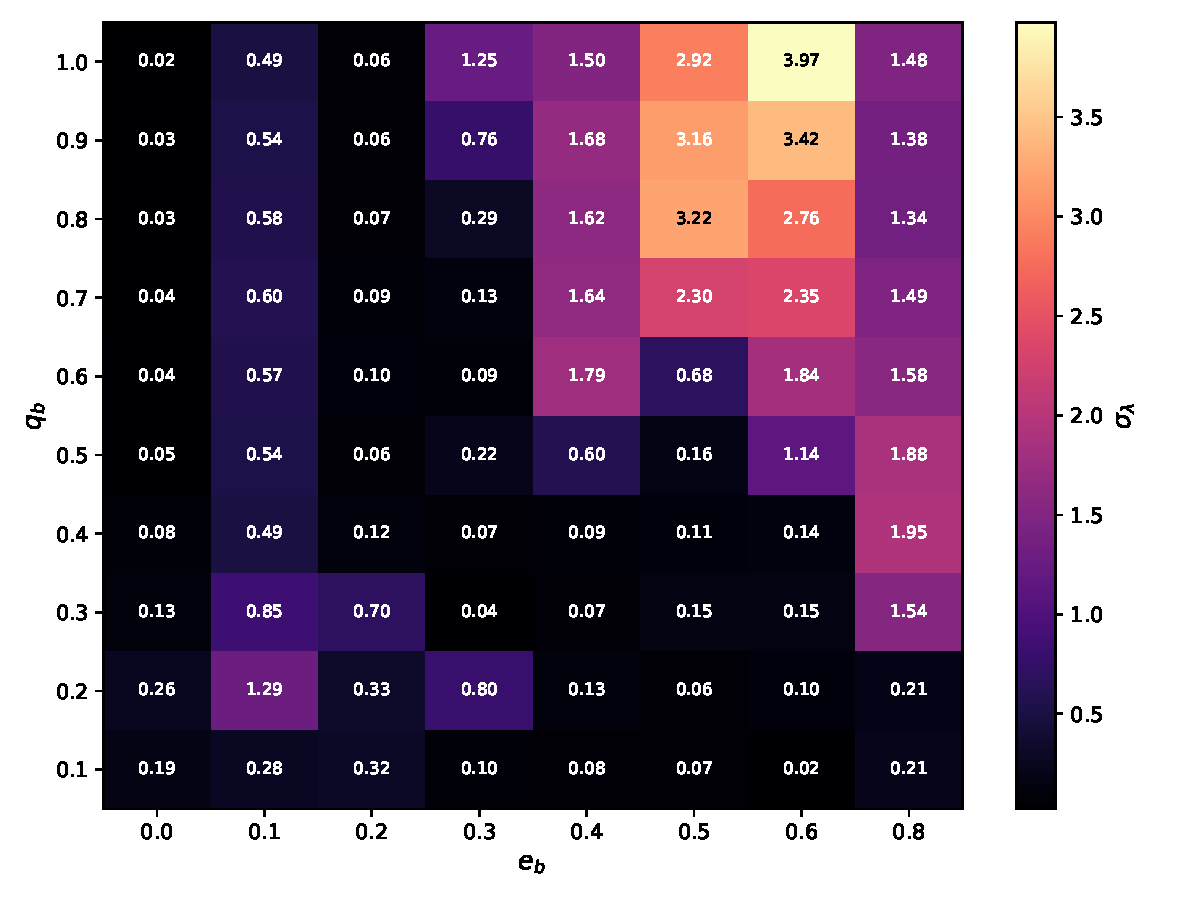
\includegraphics[width=1\linewidth]{lambda_std_colormap.pdf}
    \caption{A heat-map displaying $\sigma_{\lambda}$, the standard deviation of $\lambda(t)$, to indicate the difference in oscillation behavior across our simulations.}
    \label{fig:lambda_std_heatmap}
\end{figure}

In \autoref{fig:lambda_std_heatmap} we display a heat-map indicating the variability of $\lambda(t)$. The cell values are colored according to the standard deviation of $\lambda(t)$\footnote{For our calculations of the behavior of $\lambda(t)$ we make a cut at $3000$ orbits, to not let the initial time-instability of the disk \citep{DeLaurentiis25} influence our metrics.} ---$\sigma_{\lambda}$. We note that while many of our simulations have small $\sigma_{\lambda}$ since they are time-stable (see \autoref{tab:stable_varying_grid}), those that display meaningful $\sigma_{\lambda}$ suggest a modest trend. Namely, we find that $\sigma_{\lambda}$ seems to increase with $e_b$, peaking at $e_b = 0.6$. This modest increase in $\sigma_{\lambda}$ with $e_b$ is reminiscent of \autoref{fig:a_e_cav_heatmap}, Figure 18 of \citet{DeLaurentiis25}, which indicates that the eccentricity of the cavity increases with $e_b$ and peaks at $e_b = 0.6$. This correlation further suggests that the CBD is a crucial regulator of preferential accretion.

In addition to temporal nature of $\lambda(t)$ we also comment on the mean value of $\lambda(t)$, determining which BH is preferred to accrete and to what extent. We report our results in \autoref{fig:mean_lambda_lines} and \autoref{fig:lambda_mean_heatmap}.


\begin{figure}
    \centering
    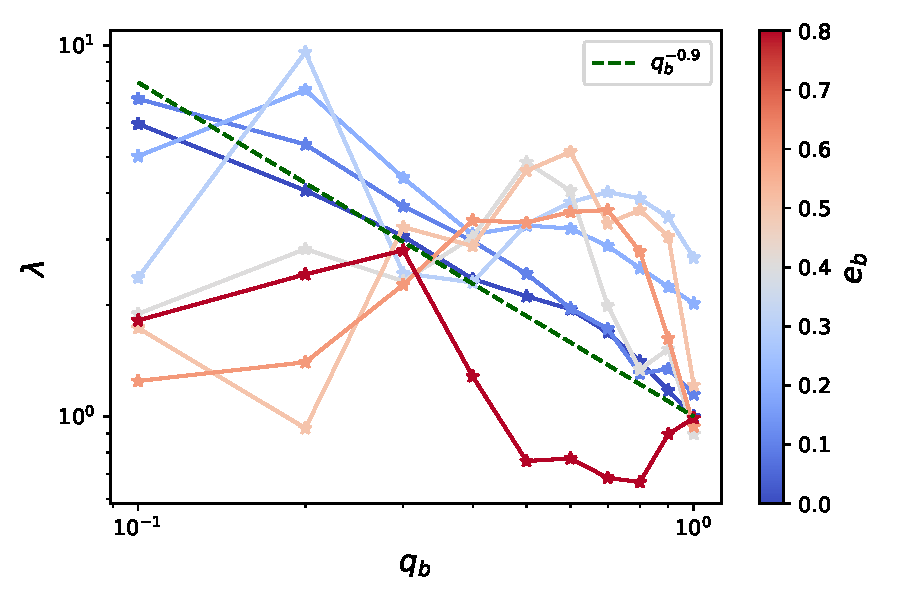
\includegraphics[width=1\linewidth]{magda_fig2.pdf}
    \caption{$\langle \lambda \rangle$ across $q_b$ and $e_b$. $\langle \lambda \rangle$ is represented on the y-axis, $q_b$ is on the x-axis, and the color represents $e_b$. We also plot the power law fitting to $\langle \lambda \rangle$ of $q_b^{-0.9}$ from \citet{siwek_prefacc} in the dashed green line.}
    \label{fig:mean_lambda_lines}
\end{figure}


\begin{figure}
    \centering
    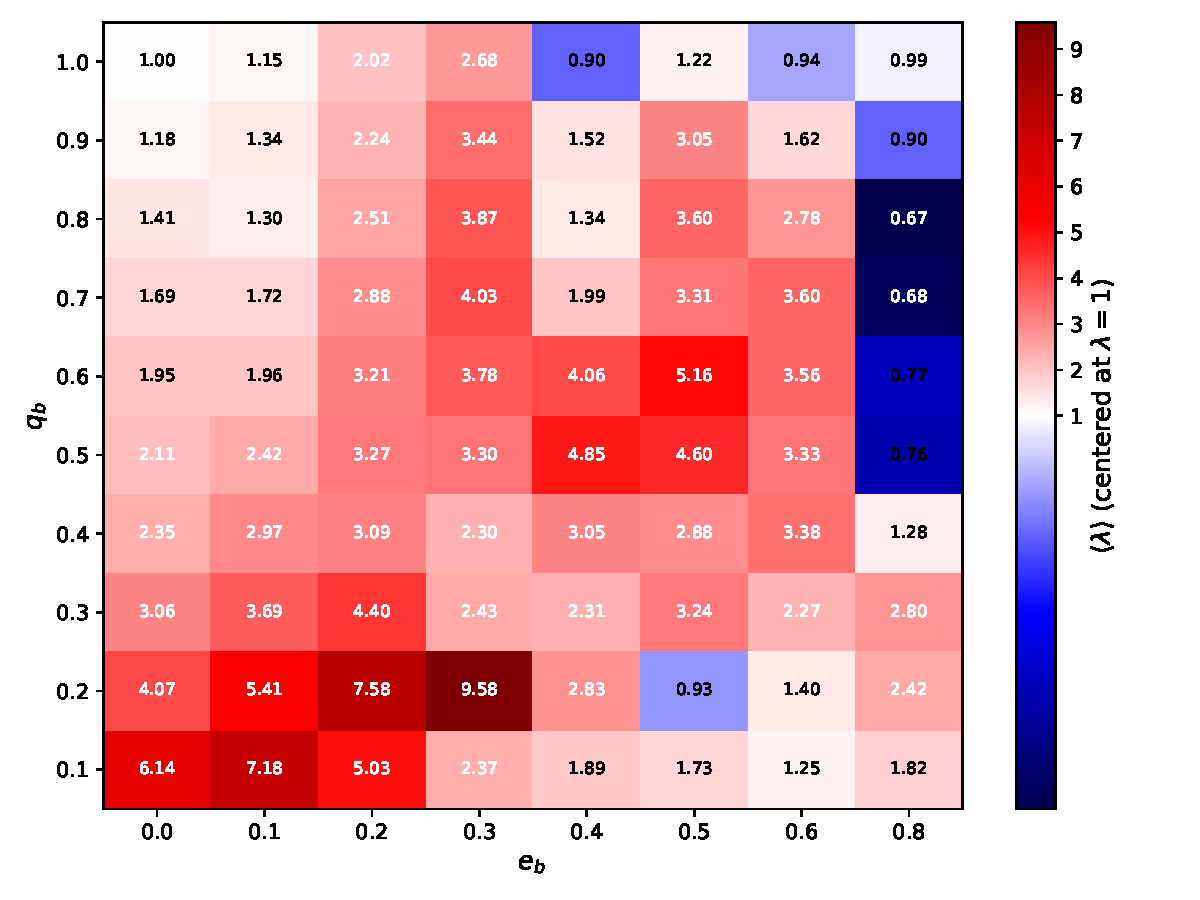
\includegraphics[width=1\linewidth]{lambda_mean_colormap.pdf}
    \caption{A heat-map displaying the time average of $\lambda(t)$ $\langle \lambda \rangle $ across our simulations. More eccentric, more unequal mass binaries seem to accrete more preferentially, though the trend is not monotonic.}
    \label{fig:lambda_mean_heatmap}
\end{figure}

In \autoref{fig:mean_lambda_lines} we display the mean values of $\lambda(t)$ on the y-axis and the $q_b$ on the x-axis, while the color represents the $e_b$. We find that our figure is in broad agreement with Figure 4 of \citet{siwek_prefacc}. We too find that the $\langle \lambda \rangle$ of the $e_b=0$ simulation seems to follow the power law of $q_b^{-0.9}$. However, we also find that $e_b=0.1$ also holds true to this line, suggesting that the behavior of $\langle \lambda \rangle $ is generic to lower eccentricity binaries and not unique to $e_b=0$. Further, we note that all our unequal-mass simulations suggest that if there is preferential accretion it is always to the secondary BH. This is in line with all the results of the literature \citep{munoz_miranda_lai_19, duffell_dorazio_2020, farris_2014, Dittmann_Ryan_21, siwek_prefacc}. Despite preferential accretion being biased towards the secondary, we note that the extent to which one BH accretes over the other depends greatly on the binary parameters. The behavior of $\langle \lambda \rangle $ is perhaps best shown in \autoref{fig:lambda_mean_heatmap}.

\autoref{fig:lambda_mean_heatmap} display $q_b$ on the y-axis and $e_b$ on the x-axis, plotting the value of $\langle \lambda \rangle $ according to color. On first glance, it is clear that some binary parameters lend themselves to stronger preferential accretion rates ($\langle \lambda \rangle$) than others. Namely, in \autoref{fig:lambda_mean_heatmap} we find that low $e_b$ and low $q_b$ values display high preferential accretion values, while high $e_b$ and high $q_b$ display lower ones as discussed in \citet{siwek_prefacc}. This is the opposite of the trend we saw for $\sigma_{\lambda}$ values in \autoref{fig:lambda_std_heatmap} and for the eccentricity of the CBD \citep{DeLaurentiis25}. This suggests that the binary parameters themselves are more important than the CBD in regulating the level of preferential accretion.


While there is certainly a trend, the level of preferential accretion is by no means monotonic with respect to $q_b$ and $e_b$. We note that intermediate values (e.g $e_b, q_b= (0.4,0.4) \, , (0.5,0.5)$) have higher preferential accretion levels than their neighbors. Further, \autoref{fig:lambda_mean_heatmap} displays interesting ``hotspots'' of high preferential accretion, with $e_b=0.3$ $q_b=0.2$ being the simulation with the highest levels of preferential accretion. We also find curious dimspots where the accretion onto both BHs is near-equal despite the binary having unequal mass. Notably, $q_b=0.2$ $e_b=0.5$ has a $\langle \lambda \rangle = 0.93$.

More importantly, we would like to note a point of deviation from \citet{siwek_prefacc}. In \autoref{fig:mean_lambda_lines} and \autoref{fig:lambda_mean_heatmap} we report $\langle \lambda \rangle \neq 1$ for $e_b, q_b =(0.2, 1.0), \, (0.3, 1.0)$ simulations. The $e_b=0.2, \, q_b = 1.0$ simulation in \citet{siwek_prefacc} had a numerical error, resulting in a deviation in $\lambda$. Accounting for this, we determine that for $e_b, q_b =(0.2, 1.0), \, (0.3, 1.0)$ simulations, the binary, in fact, preferentially accretes onto one of the BHs. The implications of this are further discussed in \autoref{sec:mass_ratio} and \autoref{sec:observations}.

Clearly, there is a variability in both the time behavior of preferential accretion and its value across simulations. In the following section we make a preliminary attempt to understand preferential accretion as an effect of the unique geometry between the binary and the CBD.

\subsubsection{Preliminary Analysis}\label{sec:preliminary_analysis}

In \autoref{sec:pref_acc} we noted similarities between the preferential accretion behavior $\lambda(t)$ and the CBD geometry. The delineation of time-stable and time-varying $\lambda(t)$ in \autoref{tab:stable_varying_grid} was likened to the precessing and locked circumbinary disks. $\sigma_{\lambda}$ seemed to display the same trend with $e_b$ and $q_b$ as that of the CBD eccentricity. While alternative explanations have been proposed \citep{Artimowicz_83_og_polish}, the assumption that the preferential accretion of the binary is related to the relative closeness of the components to the CBD's inner edge \citep{Rafikov_16_accretion, farris_2014} has been left unchallenged. In the following section we provide a first, preliminary, analysis of this assumption and alternative ways in which the CBD would influence preference accretion.



\begin{figure}
    \centering
    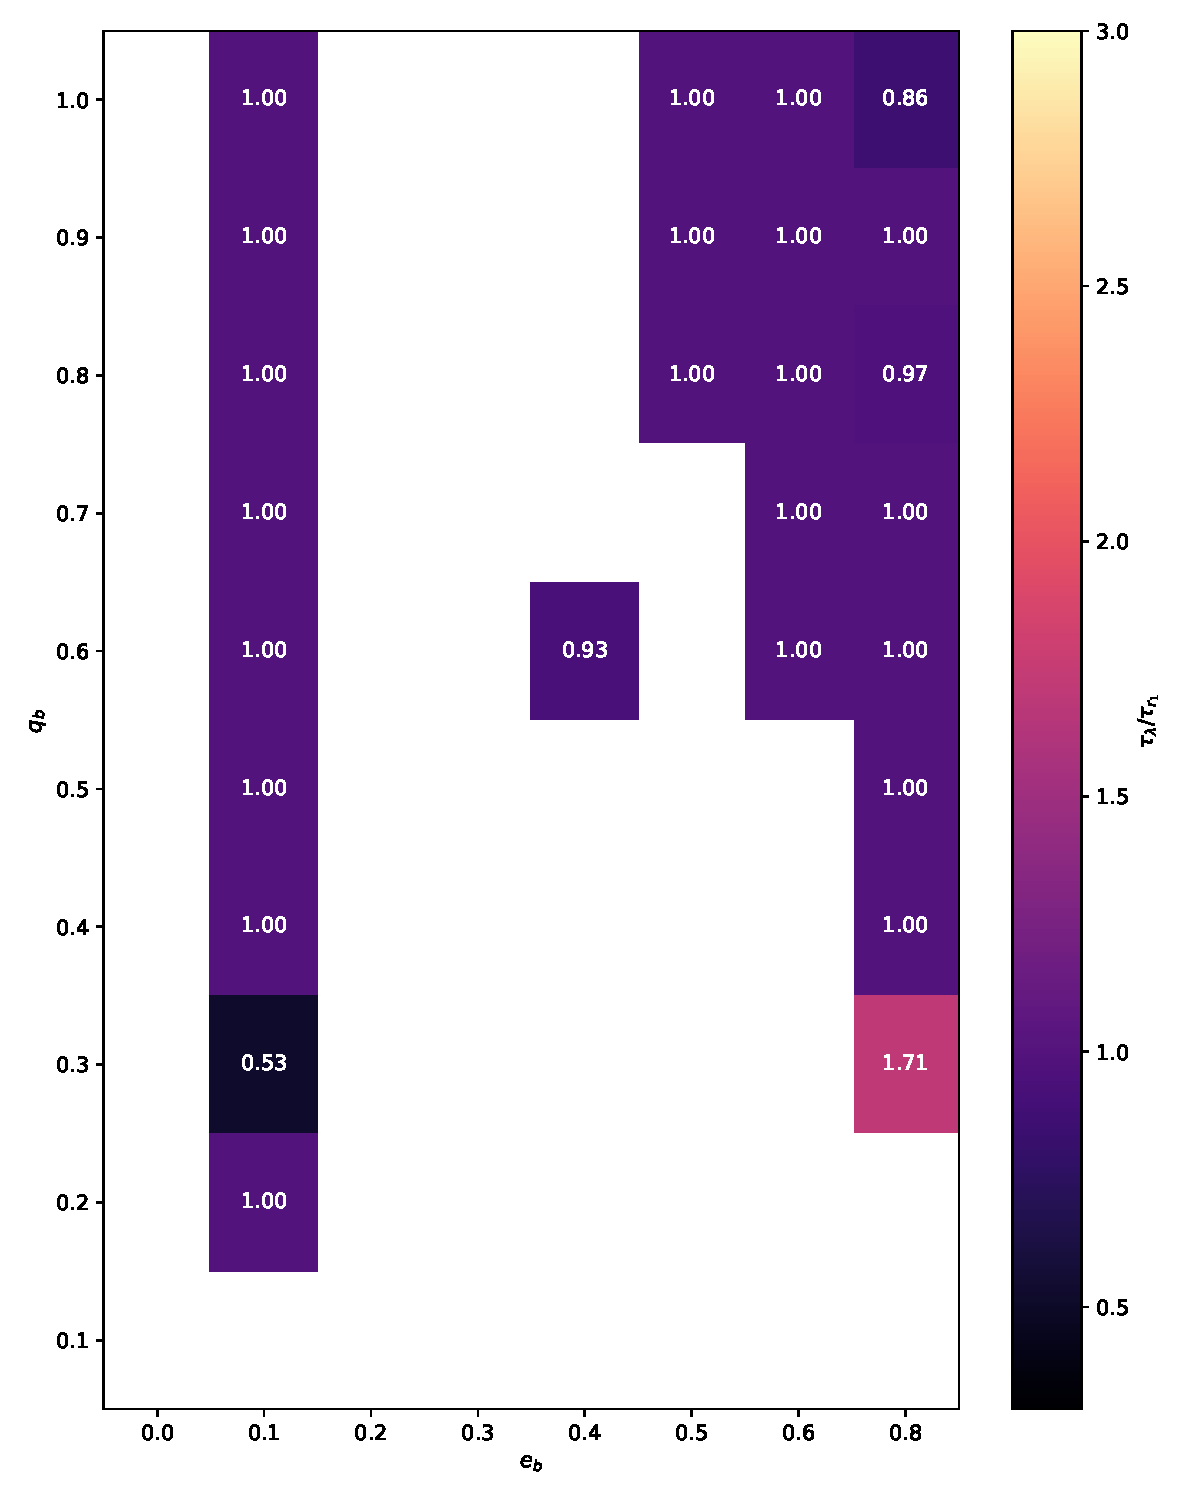
\includegraphics[width=1\linewidth]{rmin_lambda_peak_ratio._paper_ready.pdf}
    \caption{The ratio of the period of preferential accretion ($\tau_\lambda$) to the period of the CBD precession, $\tau_{r_1}$. The x-axis is the eccentricity of the binary, the y-axis is the mass-ratio of the binary, and the color of the cells correspond to the ratio of the periods. The uncolored cells are those where a period for $r_1$ or $\lambda$ could not be determined.}
    \label{fig:rmin_lambda_peak_ratio}
\end{figure}


As discussed in \autoref{sec:methods}, we use the dominant Fourier modes of the cavity to reconstruct its shape as a function of $\theta$: $r_{\rm{cav}}(\theta)$. Combined with the position of the BHs, we then define the distance from the inner edge of the CBD, ``the cavity wall'', to each BH as a function of $\theta$. We take $\theta_1^*$ and $\theta_2^*$ such that $r_{\rm{cav}}(\theta)$ is minimized for each BH. We then calculate $r_{1} = r_{\rm{cav}}(\theta_1^*) -r_{\rm{BH}_1}$ and $r_{2} = r_{\rm{cav}}(\theta_2^*) -r_{\rm{BH}_2}$ where $r_1$ and $r_2$ are the closest distances from the cavity-wall to the primary and secondary BH, respectively. Since our BH positions are fixed---as we only record snapshots at apocenter---$r_1$ and $r_2$ simply encode the information about the size and orientation of the CBD and serve as proxies.

A first step in determining the relationship between preferential accretion and the CBD is to study the temporal behavior. We have already determined that, except for the $e_b = 0$ case, all precessing CBDs result in a non-time stable $\lambda(t)$. $r_{1}(t)$ and $r_{2}(t)$, proxies for the CBD orientation, display the same split into time-stable and time-varying behavior as $\lambda(t)$ in \autoref{tab:stable_varying_grid}. For simulations with time-varying $\lambda(t)$ we compare their period of oscillation with that of $r_{1}$ and $r_{2}$. To determine the period of each time-series we first calculate a fast Fourier transform (FFT) and normalize the amplitudes by their sum. The period is the defined at that of the largest amplitude in the spectrum which has a normalized value $>0.05$. We find the periods of $r_1$\footnote{It is important to note that we have found the period of $r_1$ and $r_2$ to be exactly equal in all our simulations, making either appropriate for this calculation.} and $\lambda$ in this fashion and display the ratio of the two periods in \autoref{fig:rmin_lambda_peak_ratio}.

We note that the ratios reported in \autoref{fig:rmin_lambda_peak_ratio} are nearly all equal to one. Though certain binaries have ratios that deviate from unity we note that upon further investigation these deviations do not suggest resonances between CBD precession and preferential accretion but rather point to the difficulty of FFT to handle periodic, non-sinusoidal $\lambda(t)$ for such simulations (e.g $e_b =0.4$, $q_b = 0.8$). Thus, we find that the precession of the CBD determines not only whether $\lambda(t)$ varies but also the period at which it varies.

\begin{figure}
    \centering
    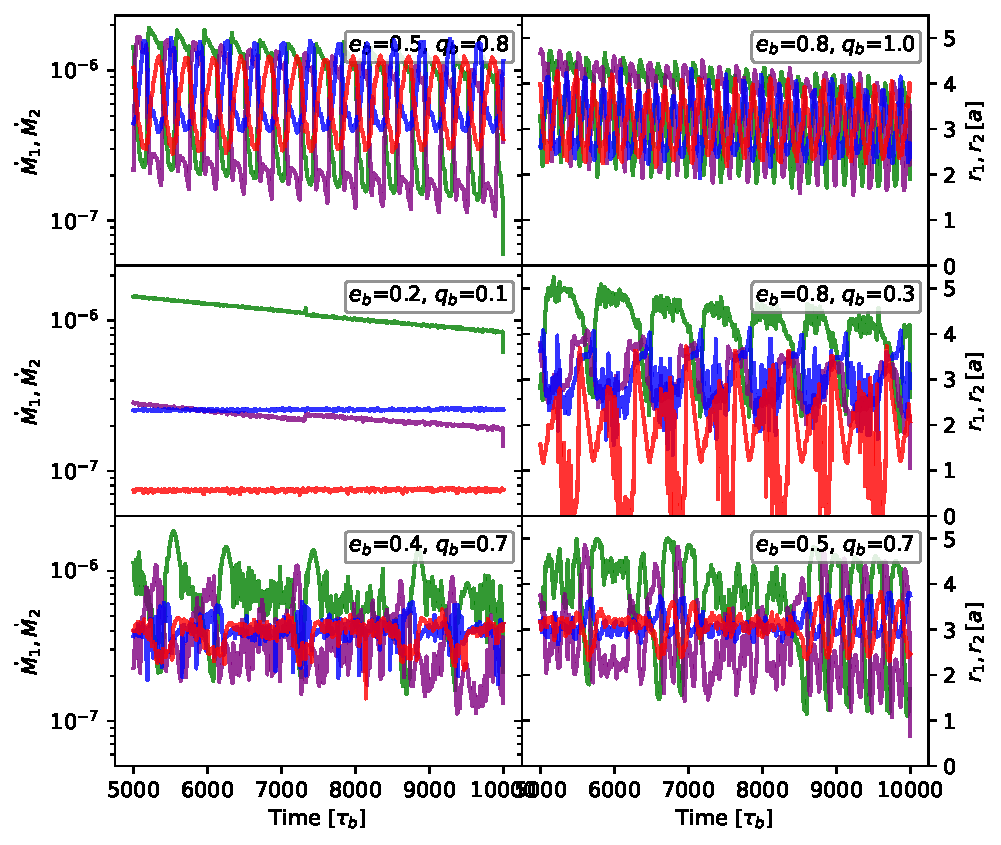
\includegraphics[width=1\linewidth]{proof_of_lambda_r_not_causal.pdf}
    \caption{Comparison between the time-series of $\lambda(t)$ (black), $r_1(t)$ (blue), and $r_2(t)$ (red). Clockwise from upper left we display $e_b, q_b = (0.5, 0.8)$, $(0.8, 0.3)$, $(0.4,0.7)$, $(0.5,0.7)$, $(0.2,0.1)$, and $0.8, 1.0$. We find that the BHs position with respect to the cavity does not determine the components' relative accretion rates.}
    \label{fig:lambda_rmin_panels}
\end{figure}

In \autoref{fig:lambda_rmin_panels} we display $r_1$ (blue) $r_2$ (red) and $\lambda$ (black) for a slice in time for six of our simulations, with the dual y-axis representing the  dimensionless lambda value (left) and the distance from each BH to the edge of the cavity in units of $a$ (right).

As indicated by \autoref{fig:rmin_lambda_peak_ratio} the variability of the distance from the BHs to the cavity displays the same period (or lack thereof) as $\lambda$. This is abundantly clear for the simulations in the left column of \autoref{fig:lambda_rmin_panels}, however we note that it is also true for some of the simulations in the right column where the period is time-varying. It is especially well captured by $e_b=0.5$, $q_b = 0.7$ where the change from a stochastic to periodic $\lambda$ signal at $\approx 8500 \tau$ is mirrored in the change of behavior of $r_1$, and $r_2$. Further, in $e_b=0.4$, $q_b = 0.7$ we find that large amplitude changes in $r_1$ and $r_2$  (e.g $\approx 6000 \, , 9000 \, \tau$) occur simultaneously with large amplitude changes in $\lambda$.

The naive understanding of the tie between preferential accretion and the distance to the black holes is as follows. The inner cavity rim hosts the densest, slowest-moving gas in the system \citep{shi_2012, farris_2014, duffell_dorazio_2020}. Whenever a black hole's Hill sphere overlaps that rim, the steep local gravitational-potential gradient bends incoming streamlines into its mini-disk, and the instantaneous capture rate obeys a Bondi-Hoyle-like scaling
\begin{equation}
  \dot{M}_{\rm near} \propto \Sigma_{\rm rim} \, v_{\rm rel}^{-3}.
\end{equation}
A companion farther from the rim encounters lower surface density and higher gas-BH relative velocity \citep{miranda_munoz_lai_2017, dorazio_duffel}, so
\begin{equation}
  \frac{\dot{M}_{\rm far}}{\dot{M}_{\rm near}} \sim \frac{\Sigma}{\Sigma_{\rm rim}} \left(\frac{v_{\rm rel}}{v_{\rm rel,\,near}}\right)^{3} \ll 1,
\end{equation}
suppressing its accretion by orders of magnitude even though both black holes share the same global gas reservoir.


In $(e_b, q_b) = (0.2, 0.1)$ we see what we would expect from our naive explanation. The corresponding panel of \autoref{fig:lambda_rmin_panels} shows that this simulation has a CBD that is locked such that our primary black hole (blue) is about twice as far from the cavity edge than our secondary black hole (red). Correspondingly, we see that the secondary is accreting at a rate about five times the primary, seemingly as a result of the secondary's greater pull on its neighboring portion of the CBD. In fact, we can even take this further and note the fact that the tidal potential on the gas by the secondary is about four to five times greater than its companion, the same factor difference as the accretion rate. However, our naive approximation is inherently over-simplistic. It doesn't take into account each BH's minidisk, the streams by which the gas is fed to the BH, or any non-linear fluid dynamics, such as shocks, that may be relevant in this mechanism. Studying the other panels, we see that our naive explanation no longer suffices.

All simulations displayed in \autoref{fig:lambda_rmin_panels}, except for $e_b=0.2 \, , q_b=0.1$, show that lower $r_2$ values do not correspond to higher accretion rates onto the secondary. The naive explanation suggests that $r_1$ should be exactly ``in-phase'' with $\lambda$ while $r_2$ should be exactly $\pi/2$ ``out-of-phase''. However, we find that $e_b, q_b = (0.5, 0.8)$ and $e_b, q_b = (0.8, 1.0)$ both clearly do not display such behavior. The former displays that both $r_1$ and $r_2$ are $\pi/4$ out of phase with $\lambda$, while the latter displays the exact opposite to our naive expectation, that $r_1 $ is in fact ``in-phase'' and $r_2$ is ``out-of-phase''. Further, when turning to $e_b, q_b =(0.8, 0.3)$ and $e_b, q_b = (0.4, 0.7)$ we note that our naive approximation further breaks down, as now the amplitude of $r_1$ relative to $r_2$ does not strictly coincide with one BH having preferred accretion over the other. We note that for $e_b, q_b =(0.8 , 0.3)$ while the primary is always at least as far away from the cavity-wall as the secondary, we still see periods where the primary accretes perferentially. Further, for $e_b, q_b = (0.4 , 0.7)$ we see a similar issue in that during periods where both the primary and secondary are equidistant from the cavity wall, the secondary is accreting up to 4 times more than the primary\footnote{While $\lambda$ is a ratio and this behavior could be due to small amplitude deviations in $\dot{M}_1$ and $\dot{M}_2$, we found that the amplitude of the sum is not strongly suppressed during this period.}.

From the above analysis it is clear that that the naive explanation of distance to the cavity and tidal potential is not robust. While the variability and periods of both are linked, they are far from causal. 
%Preliminary further analysis has suggested that the deviations from the behavior can be understood through the lens of ballistic trajectories and shock induced accretion. 
While this study has focused on describing the zoo of preferential accretion behaviors and its ties to the CBD, a more robust explanation on how the binary preferentially accretes will be explored in a forthcoming paper.



\subsection{Mass Ratio}\label{sec:mass_ratio}
In addition to preferential accretion, we also report the average rate of change of the mass ratio, $\langle \dot{q} \rangle$. Namely, we calculate $\dot{q}(t)$ as described in \autoref{eqn:q_dot} in \autoref{sec:methods}, make a time-cut at $3000\tau$ to ensure that early instabilities do not effect our results, and report the mean on the truncated time-series in units of $\dot{M}_b/M_b$ in \autoref{fig:qdot_heatmap}.

\begin{figure}
    \centering
    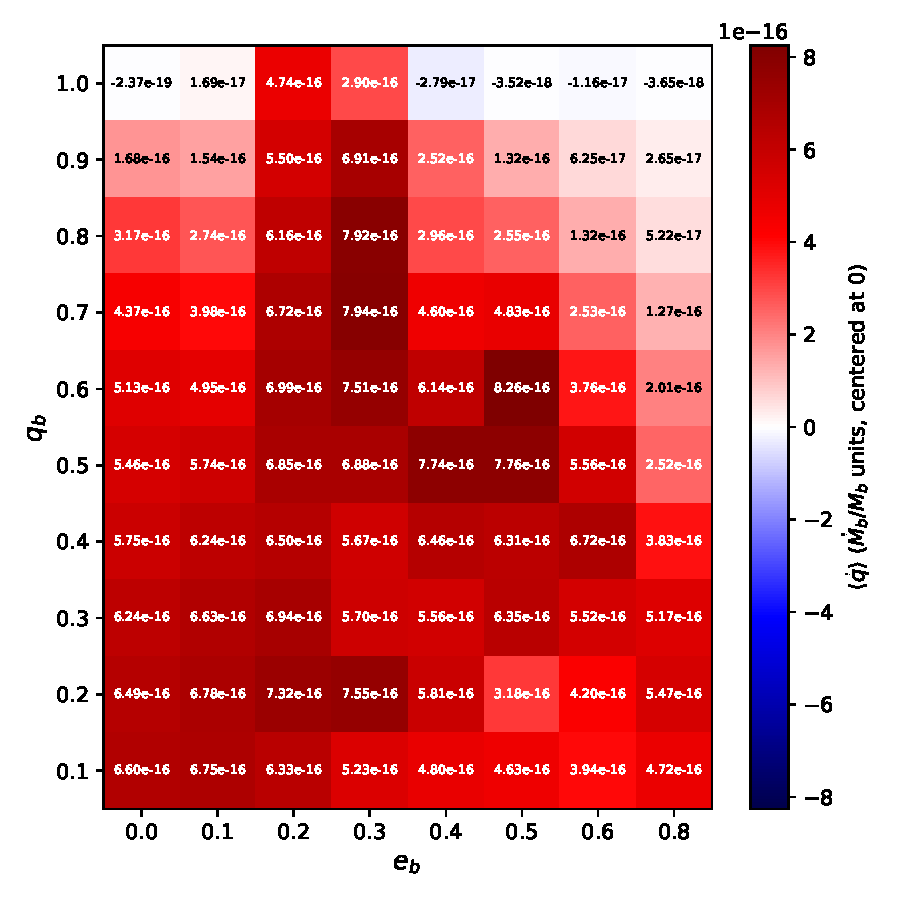
\includegraphics[width=1\linewidth]{qdot_heatmap_new.pdf}
    \caption{The average rate of change of the mass-ratio $\langle \dot{q} \rangle$ for our simulation suite. The x-axis is $e_b$, the y-axis is $q_b$, and the value of $\langle \dot{q} \rangle$ is represented as color.}
    \label{fig:qdot_heatmap}
\end{figure}

What first strikes us in \autoref{fig:qdot_heatmap} is that for all $q_b \neq 1$ simulations the binary $\langle \dot{q} \rangle$ is positive, meaning that the binary is evolving towards equal mass. We note, however, that the rate of this evolution is quite varied, spanning two orders of magnitude. Further, the gradient of $\langle \dot{q} \rangle$ in parameter space is not uniform. In fact, we see that there exists a massive drop off in $\langle \dot{q} \rangle$ in the upper right corner of \autoref{fig:qdot_heatmap}, starting along the diagonal extending from $q_b = 0.8, e_b=0.6$.

Turning to the upper row of \autoref{fig:qdot_heatmap} we find that while most of the $q_b =1$ simulations display near zero values of $\langle \dot{q} \rangle$\footnote{The negative values reported are within the standard error of the mean for the $\dot{q}$ time-series ($\approx 10^{-2}$ for $q_b =1$) and can thus be taken to be zero.} we find that there are two simulations which notably do not. Namely, the $q_b=1 \, , e_b=0.2 $ and $q_b=1 \, , e_b=0.3 $ simulations display strong positive $\langle \dot{q} \rangle$ values, meaning that the ``secondary''\footnote{In the equal-mass case, ``secondary'' and ``primary'' merely identify the components of the binary which at apocenter are in the same spatial quadrant as the secondary and primary of an unequal mass binary.} BH is growing more massive than the primary. However, since this a $q_b = 1$ case, this non-zero $\langle \dot{q} \rangle$ means that the binary is in fact being fed in such a way that it is evolving away from unity. This result for $e_b, q_b=(0.2, 1.0) $ stands as a correction to \citet{siwek_prefacc} where it was reported that $q_b$ would remain at one for this case. However, after ensuring to correctly track the sink particles in the $q_b=1$ simulations we find that accretion towards unity for SMBBHs is not necessarily a given. This makes sense especially in light of the results of \citet{DeLaurentiis25} where it was reported that the $e_b, q_b=(0.2, 1.0)$ and $(0.3, 1.0) $ simulations have stable, locked disks in line with \citet{siwek_prefacc}, with a stable non-varying $\lambda$, which in this case was coincident with the primary being further from the cavity edge than the secondary. 

The finding that equal-mass binaries at $e_b=0.2 \, , 0.3$ will accrete away from equal mass is an entirely novel result and has deep implications on CBD structure and SMBBH population statistics. Firstly, from \citet{DeLaurentiis25} we note both  $e_b, q_b=(0.2, 1.0)  $ and $(0.2, 0.9)  $ simulations have locked disks in roughly the same orientation, with the pericenter of the disk being closest towards the secondary. However, we note that the $q_b = 1$ case is accreting away from unity in such a way that the BH which was initially the ``secondary'' becomes the primary. This would likely cause the disk, which is oriented towards the secondary, to realign itself---flipping according to the switch in primary and secondary position. The details of the disk's reaction to this change in binary parameters would not only provide key insights into the mechanism behind CBD orientation, but could provide insight not only into how far away from unity the binary evolves, but depending on the process of the re-orientation could prove to be an event with characteristic EM signatures. 

\section{Observational Implications}\label{sec:observations}
In the following section we discuss the observational consequences of our $\lambda(t)$ and $\dot{q}$ results (see \autoref{sec:results}).

\subsection{Flickering Jets}

A key observational consequence of accretion onto BHs is the potential launching of jets. While the exact mechanism to launch jets continues to be an extremely active area of study, we can broadly understand jet launching through the lens of the radiative efficiency of the accretion disk. When an accretion disk is radiatively efficient the photons, and thus the energy they provide, are efficiently radiated away from the disk. However, in radiatively inefficient disk, the photons get trapped in the disk, causing a buildup of energy and pressure, both thermal and magnetic. This scenario can result in large pressure gradients that could drive jets, as well as a strong buildup in magnetic field strength which could be extracted via the Blandform-Znajek mechanism. Radiatively inefficient, geometrically thick disks are commonly found at low accretion rates $\dot{M}<0.01\dot{M}_{\rm{Edd}}$ \citep{Muryel_lowedd_jet_21} and at high accretion rates $\dot{M}>\dot{M}_{\rm{Edd}}$. Given these criteria for jet-launching we are able to make statements about the jets from our simulations.


To do so, we must first scale our numerical accretion rates, which are in units $M_{\rm{bin}}/\tau$ to Eddington units. To be able to retain information about the relative accretion rates of each BH to the other, we must set the accretion rate of the binary $\dot{M}_b \equiv \dot{M}_1 +\dot{M}_2$ to be $\gamma \dot{M}_{\rm{edd}}$ where $\gamma$ is an arbitrary scale factor and 
\begin{equation}
    \dot{M}_{\rm{Eedd}} = \frac{4\pi GM m_p}{c \eta \sigma_t}
\end{equation}
where $m_p$ is the proton mass, $\sigma_t$ is the Thomson scattering cross-section and $\eta \equiv 0.1$ is the radiative efficiency. We are then able to convert the accretion rate of each individual BH to units of $\dot{M}_{\rm{Edd}}$.

\begin{figure*}
    \centering
    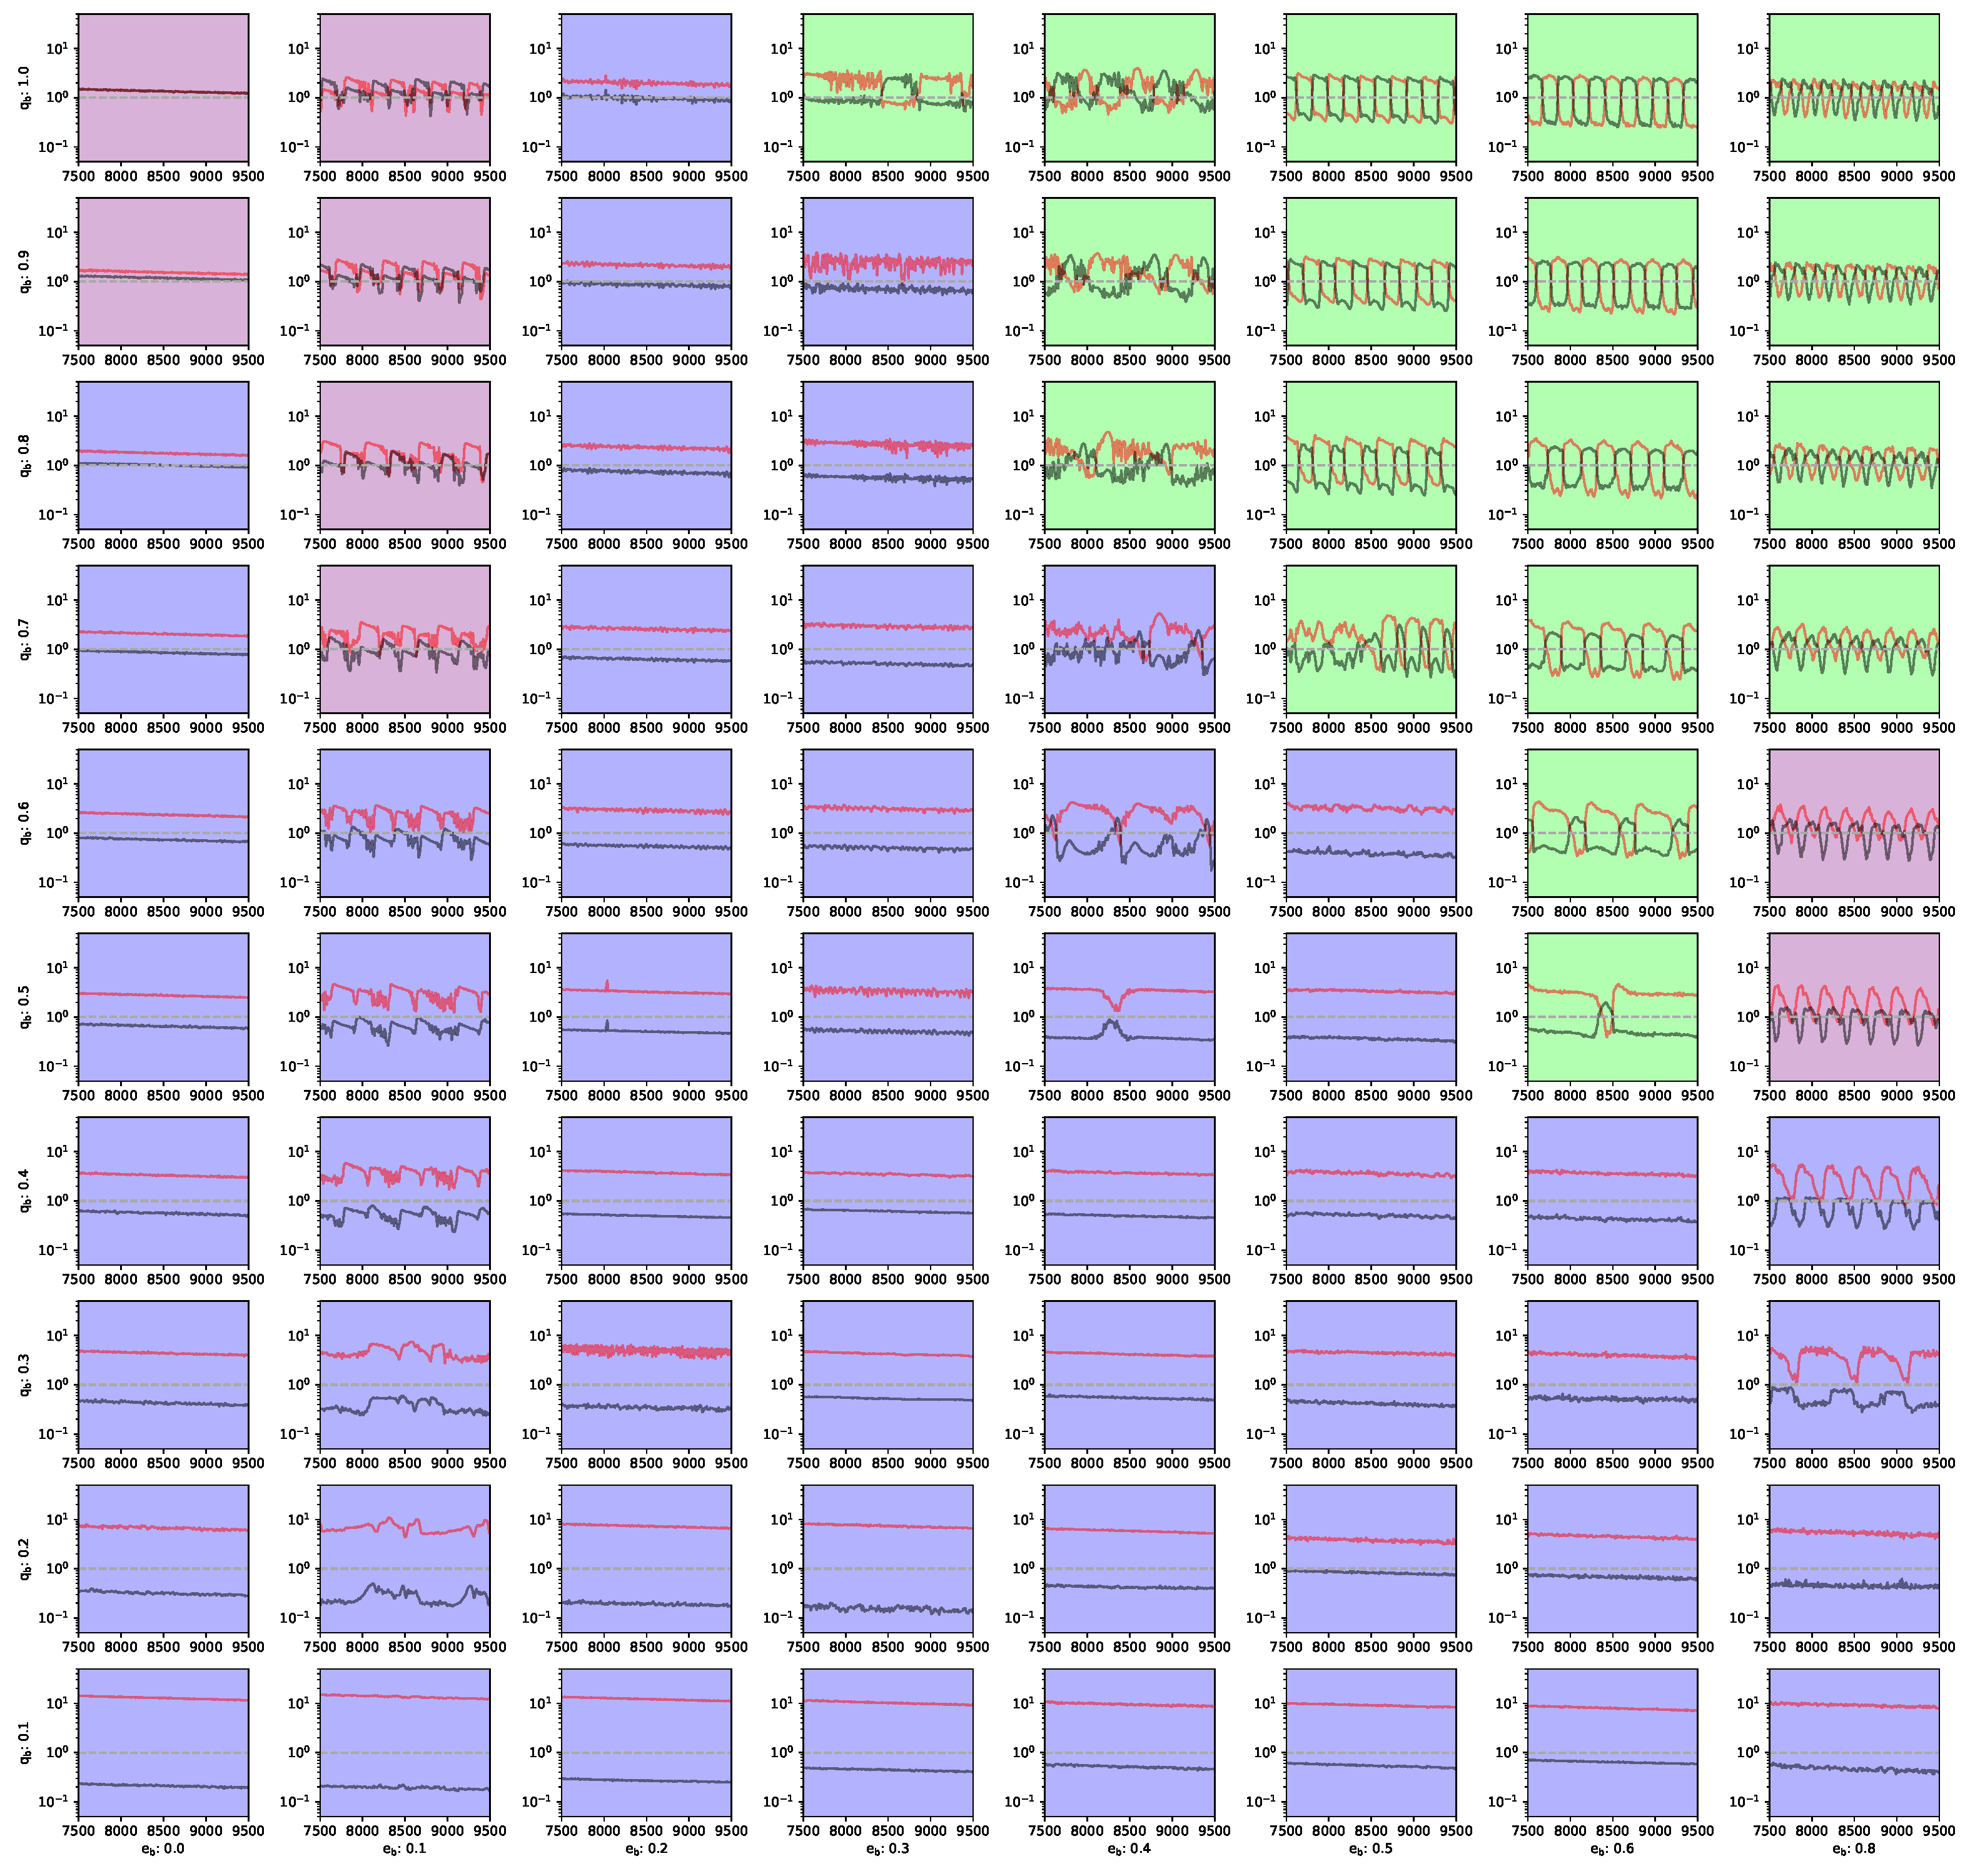
\includegraphics[width=1\textwidth]{mdot1_mdot2_1edd_both_truncated.pdf}
    \caption{Depiction of Eddington-normalized accretion rates for our simulation suite, with panel backgrounds colored by jet-regime. The panel structure is the same as that of \autoref{fig:lambda_full}, with time on the x-axis of each panel, accretion rate, in Eddington units, on the y-axis. We display the accretion rate of the primary (red), the secondary (black) and the jet-launching threshold of $1\dot{M}_{\rm{Edd}}$ (horizontal dashed gray). Blue background colors indicate single jet regimes, purple indicates dual-jet regimes, and green indicates flickering jet regimes.}
    \label{fig:mdot_edd}
\end{figure*}


\begin{figure}
    \centering
    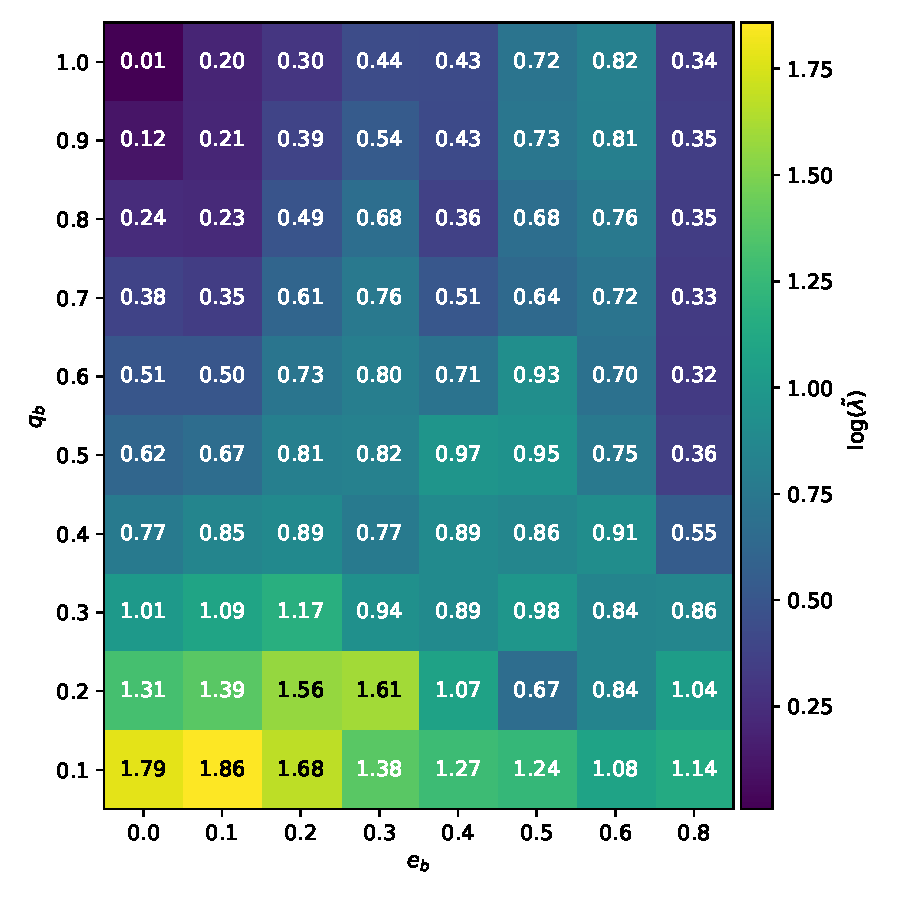
\includegraphics[width=1\linewidth]{lambda_edd_max_over_min_heatmap.pdf}
    \caption{$\tilde{\lambda}$ for our simulation suite. The x-axis is $e_b$, the y-axis is $q_b$, and the colors indicate the value of $\log (\tilde{\lambda})$.}
    \label{fig:lambda_tilde_map}
\end{figure}


In \autoref{fig:mdot_edd} we set the accretion rate of the binary to be $1 \dot{M}_{\rm{Edd}}$ assuming a $10^{7} M_{\odot}$ binary and plot the accretion rate for both BHs normalized to their respective Eddington accretion rates. The horizontal gray dashed line is at $1\dot{M}_{\rm{Edd}}$ to represent the accretion rate above which which jets are likely to launch. The red lines represent the accretion rate of the secondary, and the black lines represent the accretion rates of the primary. The background color of the panel is associated with different jet-behaviors: purple for dual jets, blue for a single jet, green for flickering jets. The time-slice displayed is arbitrary and serves to merely highlight the accretion behavior.

What first strikes us in \autoref{fig:mdot_edd} is the wide variety of difference in magnitude between the two BHs' accretion rates. Since the Eddington accretion rate scales linearly with the BH mass we expect that the accretion rates of the secondary to be increased greatly when normalized to Eddington units. This is evidenced by the nearly 2 order of magnitude difference between the secondary and primary at $q_b=0.1$. Further, we also notice that the behavior of the individual accretion rates of the black holes are quite varied, as the $\lambda(t)$ results suggested. Aside from the differences in whether the BHs' accretion rates are stable or not, the profile of the accretion rate itself is varied. Some binaries experience accretion rates that are close to sinusodial (e.g $e_b=0.6, 0.8$), others seem to closer resemble square-waves (e.g $q_b=1, e_b=0.3, e_b=0.5$), others yet have quite sharp breaks that evade simple characterizations (e.g $e_b=0.1$, $q_b=0.7$). Further, we note that the accretion rate of one BH is not always simply the accretion rate of the other with a different baseline and $\pi/2$ phase shift. Rather, they can take on notably different profiles from each other, resulting, at times, in both BHs experiencing a local peak in accretion rate, but because of different accretion rate amplitudes result in a peak in $\lambda$. It is exactly this zoo of individual BH accretion rates, and the way in which they compare to each other, that yield an interesting assortment of jet-launching behaviors.

In \autoref{fig:mdot_edd} we delineate three broad regimes: a) binaries where one BH launches a jet (blue), b) binaries where both BHs coincidentally launch jets in a sustained and repeated fashion (purple), c) binaries where both BHs launch jets in a successive, alternating fashion (green). We describe these jet-behavior regimes as single jets, dual jets, and flickering jets, respectively. We assigned jet-regimes by determining whether the accretion rate of each BH surpassed a threshold value of $1.1\dot{M}_{\rm{Edd}}$ for greater than $50 \tau$, and whether those instances were temporally coincident for greater than $50 \tau$. 

We note that the majority of simulations at the assumed binary accretion rate of $1\dot{M}_{\rm{Edd}}$ are single-jet systems, where most of them have low $q_b$ due to the highly unequal Eddington-normalized accretion rates of those systems. 

The flickering jet systems are clustered at higher $q_b$ and $e_b$. Due to large $\lambda$ amplitudes, such systems are able to exist up to $q_b=0.5$. It is important to note that since these flickering jets are dependent on large $\lambda$ oscillations they are unique to $e_b \neq 0$ binaries.

Finally, we have a few dual-jet systems. For those at $e_b=0$ both BHs accrete at nearly the same, stable rate and thus both launch sustained jets. However, we also note that we have dual jets for binaries whose $\lambda \neq 1$. We note that the dual-jet systems at $e_b=0.1$ and $e_b=0.8$ show both BHs having coincident, local peaks in accretion rates, meaning that the binary sustainably and periodically launches two jets.

While dual jets have been suggested before \citep{Palenzuela_dualjet_10, Qian_dualjet_19} and have even been simulated \citep{Gutierrez_24, Ressler_dualjet_25}, we believe that we are \textit{the first to report evidence suggesting a flickering-jet behavior}. An entirely new regime, it not only provides a unique observational determination of eccentric binaries but it is also a uniquely distinct kind of feedback mechanism that could be further explored in cosmological simulations. 

\autoref{fig:mdot_edd} and its discussion assumed a binary accretion rate of $1\dot{M}_{\rm{Edd}}$. However, such assumption only controls the baseline of the binary accretion rate. While a different assumed binary accretion rate would not change the profiles nor the relative accretion rates of the components, it would affect the absolute amplitude---changing its jet-launching behavior.

 \autoref{fig:lambda_tilde_map} displays $\tilde{\lambda}$, which can be written as
\begin{equation}
    \tilde{\lambda} \equiv \frac{\langle \max (\dot{M}_{1} \dot{M}_{2}) \rangle }{\langle \min (\dot{M}_{1}, \dot{M}_{2}) \rangle}
\end{equation}
where $\max $ and $\min$ are element-wise functions and the accretion rates are provided in Eddington units.

The result $\tilde{\lambda}$ is dimensionless and provides the ratio of the maximum and minimum Eddington-normalized accretion rates of the binary components. Given the time-variability of $\lambda$ in \autoref{tab:stable_varying_grid} and a binary accretion rate, $\tilde{\lambda}$ can then be easily used to determine whether one or both BHs launch a jet, and whether they are temporally coincident. Namely, one can use
\begin{equation}
    \dot{M}_1 = \frac{\dot{M}_b}{\tilde{\lambda} + 1}
\end{equation}
to find the accretion rate of the primary based on the scaling of $\lambda$ and $\dot{M}_b$.
With \autoref{fig:lambda_tilde_map} in hand we are able to gain insight into the jet behavior of any proposed BBH system as a function of $q_b$ and $e_b$. Given the clustering of jet-behavior in $q_b$-$e_b$ parameter space, determination of whether a system has sustained dual jets, flickering jets, or a single jet could greatly constrain the orbital parameters of the system.

\begin{figure}
    \centering
    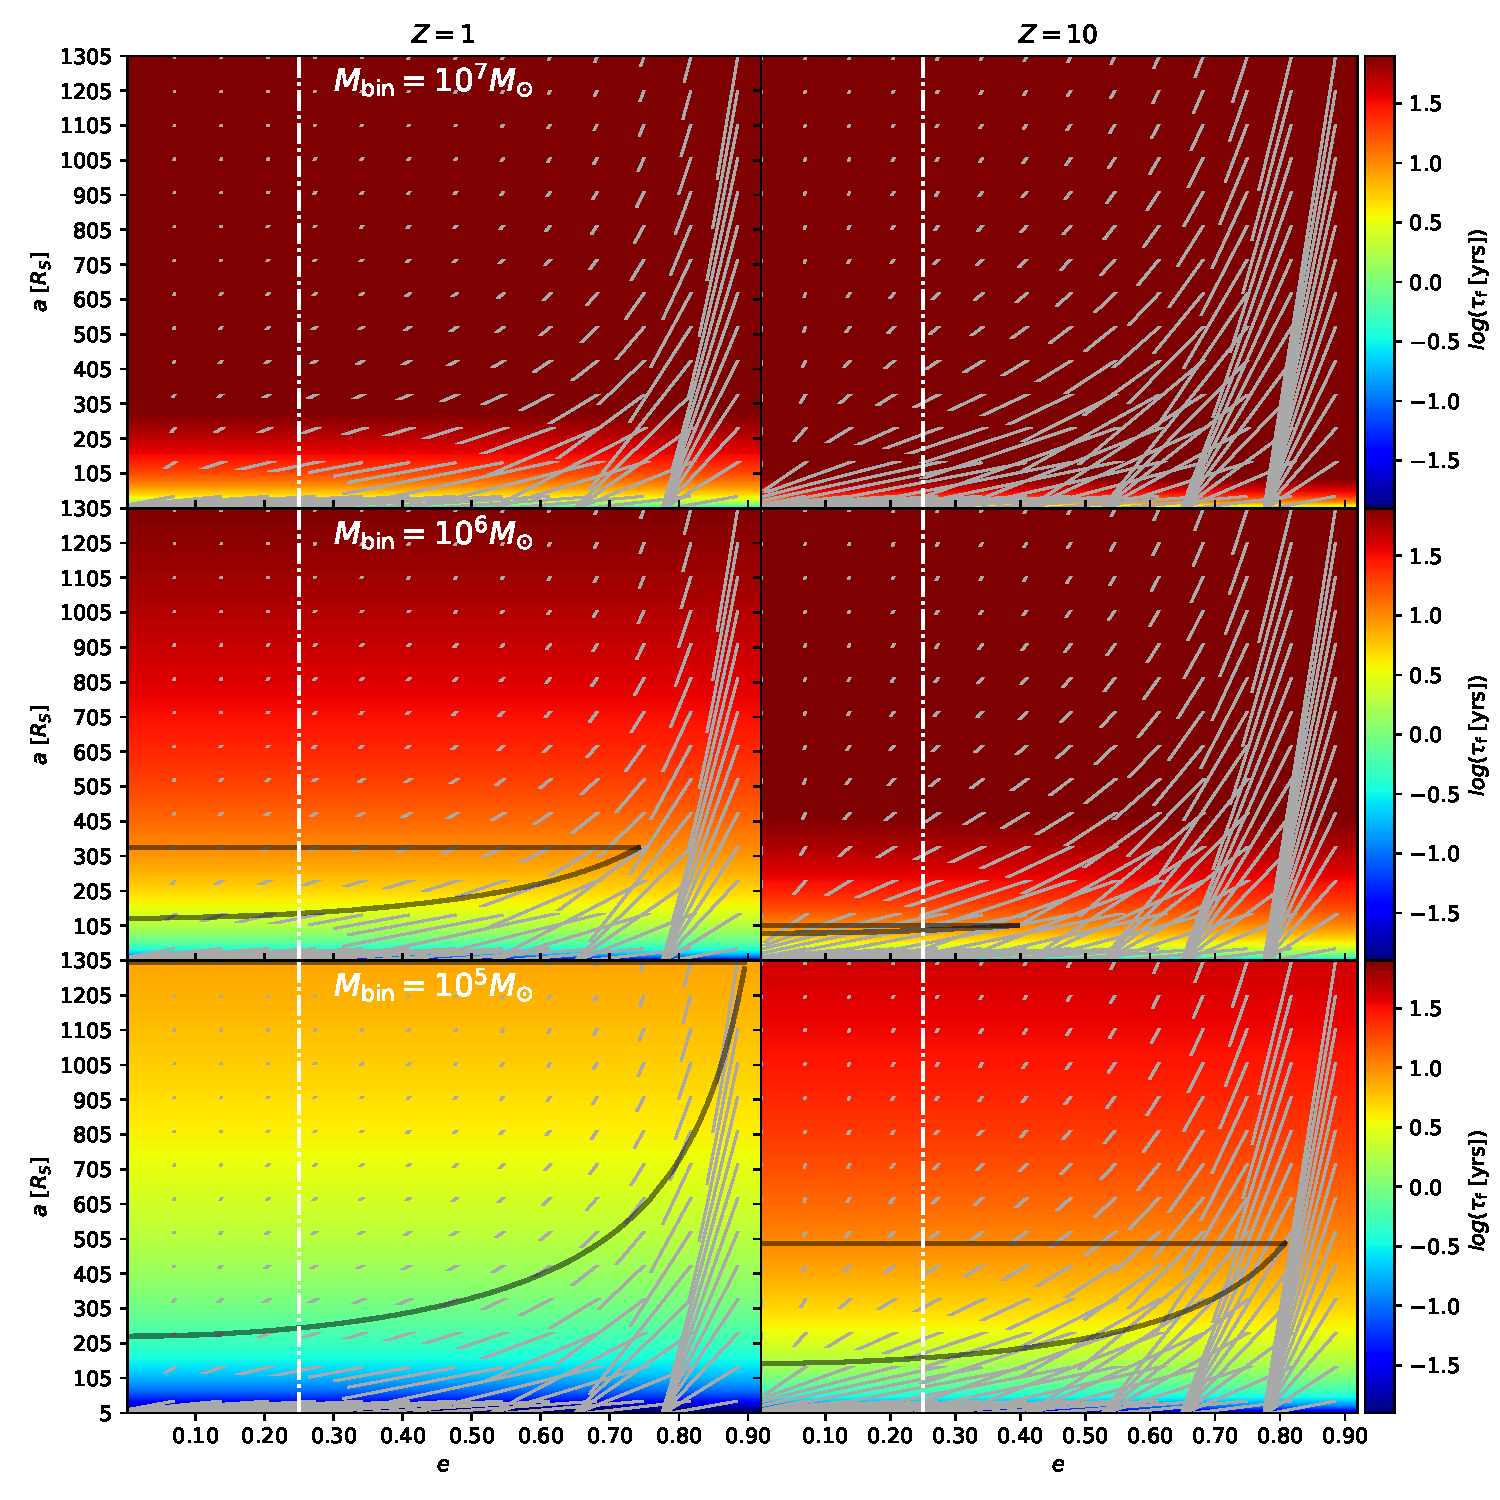
\includegraphics[width=1\linewidth]{new_obs_heatmap_new_big.pdf}
    \caption{The region of parameter space that satisfies the above time constraints (within black lines) for various binary masses at various redshifts. The x-axis of each panel is the eccentricity $e_b$, the y-axis is the $a_b$ in Schwarzchild radii, and $\tau_f$ is reported in the observer frame. The gray lines represent the net effect of 10 orbits of GW radiation on the eccentricity and semi-major axis of each BBH.}
    \label{fig:timescales}
\end{figure}


``Flickering jets'' are a unique EM signature for BBHs. In order to use them to find BBH systems, we must ensure they ``flicker''--- i.e switch which BH is preferentially accreting---on a human time-scale. In the following we compute  and place constraints on the time to ``flicker.''

Firstly, we require that the time to flicker $\tau_f$ be fewer than $10$ years in the observer's rest-frame, so that a few cycles could be possible in a human lifetime. For simplicity, we assume the flickering period is $300 \tau$. We also require that the binary not merge in less than $100$ years, in order to ensure that these systems are common enough. 

In \autoref{fig:timescales} we display the region of parameter space that satisfies the above time constraints (within black lines) for various binary masses at various redshifts. The x-axis of each panel is the eccentricity $e_b$, the y-axis is the $a_b$ in Schwarzchild radii, and $\tau_f$ is reported in the observer frame. The gray lines represent the change in eccentricity and semi-major axis for the binary, due to 10 orbits worth of GW radiation.

\autoref{fig:timescales} shows that $10^5M_\odot$ and $10^6M_\odot$ systems both display considerable regions of parameter-space that satisfy the constraints necessary to observe the flicker, up to $z=10$. We find that the region which satisfies these constraints shrinks to zero by $z=15$ and $z=100$ for the $10^6M_\odot$ and $10^5M_\odot$ systems, respectively. This provides encouraging evidence for our ability to observe these flickering jet systems.

In addition to observing a flicker occur, we note that jets are extended emission sources and thereby provide us an ability to observe a past flicker. If we could determine a geometric separation in the structure of a helical jet, this could indicate that the emission is from a binary that flickered in the past. 


\subsection{Unequal Mass Sources}
In addition to the variety of jet launching behavior and their effects on galaxy feedback, the evolution of the mass ratio of these SMBBHs is also a key observational signature. We explore whether our findings from \autoref{fig:qdot_heatmap} suggesting that some binaries do not evolve towards equal mass in fact lead to detectable $q \neq 1$ BBH systems.

In addition to its mass-ratio, the eccentricity and semi-major axis of the binary also change as functions of $q_b$ and $e_b$ due to the CBD, we represent these as $\dot{e}_{\rm{gas}}(q_b, e_b)$ and $\dot{a}_{\rm{gas}}(q_b, e_b)$, respectively. The values for $\dot{a}_{\rm{gas}}(q_b, e_b)$, and $\dot{e}_{\rm{gas}}(q_b, e_b)$ were also calculated for this full simulation suite and are reported in Figure 2 and 3 of \citet{siwek_cbdorbevol}, respectively. Since our simulation suite is discretized in $e_b$ and $q_b$ space, we define $\dot{e}_{\rm{gas}}(q_b, e_b)$, $\dot{a}_{\rm{gas}}(q_b, e_b)$ and $\dot{q}(q_b, e_b)$ as sets of piecewise functions with constant values that are centered at the binary parameter values and extend to the midpoint between it and its neighboring, sequential, binary parameter value. For example,
\begin{equation}
    \dot{q} =1.041 \,
    \begin{cases} 
     0.15 \leq q_b < 0.25 \\
      0.15 \leq e_b < 0.25 \\
\end{cases}
\end{equation}

However, in addition to CBD effects, the GWs radiated from the system also circularize and shrink the binary we include these effects through the terms
\begin{equation}
    \dot{a}_{\text{GW}} = \frac{-64 G^3 M^3 q \, f(e)}{5 c^5 a^3 (1+q)^2}
\end{equation}
and
\begin{equation}
    \dot{e}_{\text{GW}} = -e\frac{ 304 G^3 M^3 q \left( 1 + \frac{121}{304} e^2 \right)}{15 c^5 a^4 \left( 1 - e^2 \right)^{5/2} (1 + q)^2}
\end{equation}.

Thus, we are left with the set of coupled differential equations
\begin{align}\label{eqn:num_integ}
    & \dot{a}(q_b, e_b) = \dot{a}_{\rm{gas}}(q_b, e_b) + \dot{a}_{\rm{GW}}(q_b, e_b, a_b) \\
    & \dot{e}(q_b, e_b) = \dot{e}_{\rm{gas}}(q_b, e_b) + \dot{e}_{\rm{GW}}(q_b, e_b, a_b) \\
    & \dot{q}(q_b, e_b) = \dot{q}_{\rm{gas}}(q_b, e_b) \\
\end{align}
which we numerically integrate given an initial $a_0$, $q_0$, and $e_0$.


Per \autoref{fig:qdot_heatmap}, we solve the initial value problem for two equal-mass binaries with $e_b=0.2$ and $e_b=0.3$, integrating forward for $10^4 \tau$ with $a_0 = 10^3 R_S$. The results are displayed in \autoref{fig:evolution_plot}.

\begin{figure}
    \centering
    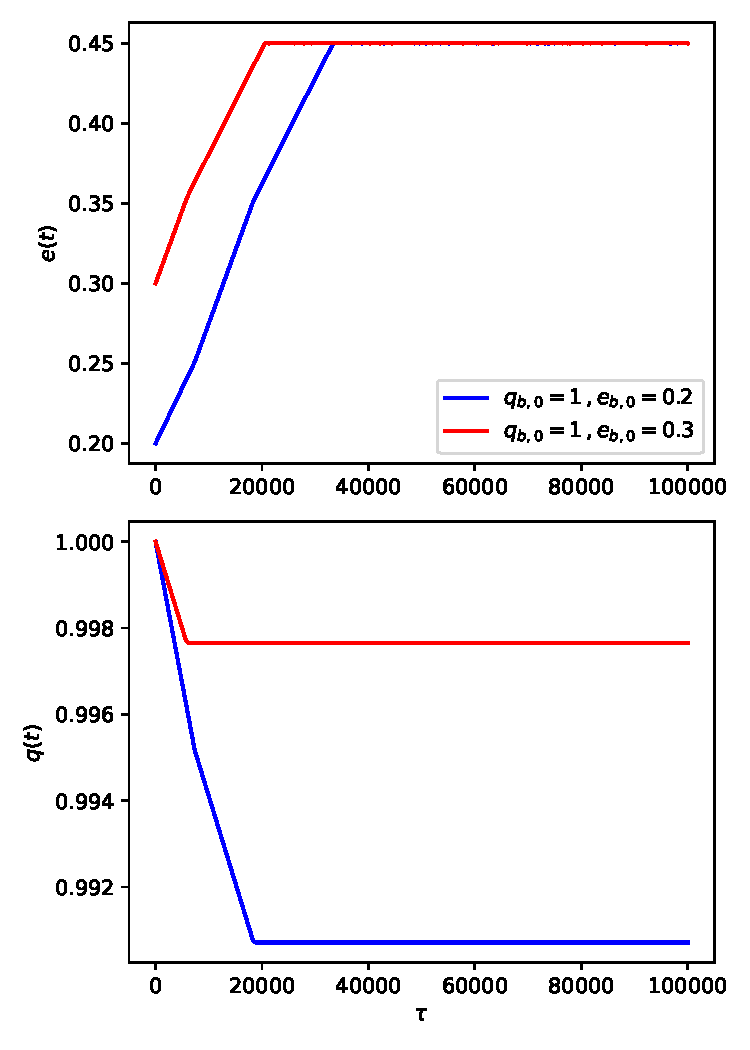
\includegraphics[width= 1\linewidth]{evolution_plots.pdf}
    \caption{Evolution of binaries away from equal-mass. We depict the result of our numerical integration of \autoref{eqn:num_integ} for $e_{b_0}, q_{b_0} = (0.2, 1.0)$ (blue) and $(0.3, 1.0)$ (red). The y-axes are $e(t)$ (upper) and $q(t)$ (lower) of the binary and the x-axes are time in units of each binary's orbital period.}
    \label{fig:evolution_plot}
\end{figure}

In \autoref{fig:evolution_plot} we display the evolution of the two binary's $e(t)$ and $q(t)$ in the upper and lower panels, respectively. Firstly, our numerical integration confirms the expectation that the binary evolves towards the expected $e_b = 0.45$ equilibrium eccentricity \citep{duffell_dorazio_2020, zrake_2021, siwek_cbdorbevol, Siwek_mbbh_pop_24}.  More interestingly, we find that the two binaries initialized at $e_b, q_b = (0.2, 1.0)$ and $(0.3,1.0)$ do indeed evolve away from $q_b=1$, and have end values\footnote{We note that} of $(0.45, 0.991)$ and $(0.45, 0.998)$, respectively. These results suggest that BBHs, which at some point in their evolution, have the parameters $(0.2, 1.0)$ and $(0.3, 1.0)$ have equilibrium mass-ratios that are not equal to one. LISA is expected to have a precision in $q_b$ of up to $0.5 \%$ \citep{Mangiagli_2020}. 
Thus, while the deviation from $q_b=1$ for the end state of $(0.3, 1.0)$ binaries may not be detectable by LISA, that of $(0.2, 1.0)$ will be will within detection limits. Thus, given enough LISA detections, a number density bump at $q<1$ could suggest the history of the binaries, indicating it passed through $(q_b=1, e_b=0.2)$.

\section{Summary and Conclusions}\label{sec:conclusion}
This paper has provided the most extensive report on the preferential accretion $\lambda \equiv \frac{\dot{M}_2}{\dot{M}_1}$ and mass ratio rate of change $\dot{q}$ for SMBBHs embedded in CBDs. In addition to calculating quantities, we provide novel insight into the behavior of these values over time and their dependence on $q_b$ and $e_b$. We also conduct a preliminary investigation into how the CBD regulates preferential accretion. We summarize our key findings below.

\begin{enumerate}
    \item Across $q_b$ and $e_b$, $\lambda(t)$ can be split into time-varying and time-stable regimes, broadly mirroring the split of the CBD into precessing and locked states. 
    \item The average preferential accretion value $\langle \lambda \rangle$ exhibits a weak positive correlation with both $e_b$ and $q_b$. The standard deviation of $\lambda$, $\sigma_{\lambda}$, exhibits a weak negative correlation with both $e_b$ and $q_b$.
    \item $\langle \lambda \rangle$ is positively correlated with more eccentric CBDs.
    \item We find strong evidence that while the CBD precession and $\lambda(t)$ oscillation have the same period, these time-series are not in phase.
    \item We do not find evidence that a BH must be closer to the CBD cavity than its counterpart, to accrete preferentially.
    \item Normalized to Eddington accretion rates, $\lambda(t)$ results in disparate accretion regimes for each BH in the binary---leading to unique jet-launching regimes. We delineate binaries that are likely to launch a sustained jet from one BH (single-jet), from each BH (dual-jet), or alternate in which BH launches a jet (flickering-jet).
    \item We find that $e_b, q_b = (0.2, 1.0)$ and $(0.3, 1.0)$ binaries do not have $q_b=1.0$ steady-states and preferentially accrete away from equal-mass. The steady-state of a $(0.2, 1.0)$ system will be detectable by LISA as having unequal mass.
\end{enumerate}

While our work has shed light on novel aspects of this system, we are still studying setups with simplified physics, namely two-dimensional hydrodynamic simulations. In future work we hope to expand this study to more physically motivated simulation setups, accounting for effects that were ignored in this study. Namely, we hope to detail $\lambda$ and $\dot{q}$ for radiation MHD simulations in three dimensions. Further, we would like to also develop GRMHD simulations for SMBBHs in order to better simulate jet-launching and test our findings on different jet regimes. In addition to developing more robust simulations, we would also like to run live-binary simulations for the $e_b, q_b = (0.2, 1.0)$ and $(0.3, 1.0)$ binary systems to not only better extrapolate how the binary evolves away from unity but to also understand how the disk reacts to the change in position of the primary and secondary. Finally, we will further investigate the mechanism behind preferential accretion, with a forthcoming analysis on the hydrodynamics of the gas within the cavity.

We conclude by noting that while the mechanism behind preferential accretion is more complex than previously thought, it is still intimately tied to the CBD and can have profound observational consequences for SMBBH systems, such as jet-launching and LISA population studies. We encourage further study into the preferential accretion mechanism and its consequences.


\section*{Data Availability}
The data underlying this article will be shared on reasonable request to the corresponding author.

\appendix
\section{}

\renewcommand{\arraystretch}{1.5} % Adjust row height

\begin{table}
\centering
\begin{tabular}{|c|c|c|c|c|c|c|c|c|} 
    \hline
    \textbf{1.0} &
    \cellcolor{blue}\textcolor{white}{P} & 
    \cellcolor{blue}\textcolor{white}{P} &
    \cellcolor{red}\textcolor{white}{L} &
    \cellcolor{blue}\textcolor{white}{P} & 
    \cellcolor{blue}\textcolor{white}{P} & 
    \cellcolor{blue}\textcolor{white}{P} & 
    \cellcolor{blue}\textcolor{white}{P} & 
    \cellcolor{blue}\textcolor{white}{P} \\ 
    \hline
    \textbf{0.9} & 
    \cellcolor{blue}\textcolor{white}{P} & 
    \cellcolor{blue}\textcolor{white}{P} & 
    \cellcolor{red}\textcolor{white}{L} &
    \cellcolor{red}\textcolor{white}{L} & 
    \cellcolor{blue}\textcolor{white}{P} & 
    \cellcolor{blue}\textcolor{white}{P} & 
    \cellcolor{blue}\textcolor{white}{P} & 
    \cellcolor{blue}\textcolor{white}{P} \\ 
    \hline
    \textbf{0.8} & 
    \cellcolor{blue}\textcolor{white}{P} & 
    \cellcolor{blue}\textcolor{white}{P} & 
    \cellcolor{red}\textcolor{white}{L} &
    \cellcolor{red}\textcolor{white}{L} & 
    \cellcolor{blue}\textcolor{white}{P} &
    \cellcolor{blue}\textcolor{white}{P} &
    \cellcolor{blue}\textcolor{white}{P} &
    \cellcolor{blue}\textcolor{white}{P} \\ 
    \hline
    \textbf{0.7} & 
    \cellcolor{blue}\textcolor{white}{P} &
    \cellcolor{blue}\textcolor{white}{P} &
    \cellcolor{red}\textcolor{white}{L} & 
    \cellcolor{red}\textcolor{white}{L} & 
    \cellcolor{blue}\textcolor{white}{P} & 
    \cellcolor{blue}\textcolor{white}{P} & 
    \cellcolor{blue}\textcolor{white}{P} & 
    \cellcolor{blue}\textcolor{white}{P} \\ 
    \hline
    \textbf{0.6} & 
    \cellcolor{blue}\textcolor{white}{P} & 
    \cellcolor{blue}\textcolor{white}{P} & 
    \cellcolor{red}\textcolor{white}{L} & 
    \cellcolor{red}\textcolor{white}{L} & 
    \cellcolor{blue}\textcolor{white}{P} & 
    \cellcolor{red}\textcolor{white}{L} & 
    \cellcolor{blue}\textcolor{white}{P} & 
    \cellcolor{blue}\textcolor{white}{P} \\ 
    \hline
    \textbf{0.5} & 
    \cellcolor{blue}\textcolor{white}{P} & 
    \cellcolor{blue}\textcolor{white}{P} & 
    \cellcolor{red}\textcolor{white}{L} & 
    \cellcolor{red}\textcolor{white}{L} & 
    \cellcolor{red}\textcolor{white}{L} & 
    \cellcolor{red}\textcolor{white}{L} & 
    \cellcolor{blue}\textcolor{white}{P} & \cellcolor{blue}\textcolor{white}{P} \\ 
    \hline
    \textbf{0.4} & 
    \cellcolor{blue}\textcolor{white}{P} & 
    \cellcolor{blue}\textcolor{white}{P} & 
    \cellcolor{red}\textcolor{white}{L} & 
    \cellcolor{red}\textcolor{white}{L} & 
    \cellcolor{red}\textcolor{white}{L} & 
    \cellcolor{red}\textcolor{white}{L} & 
    \cellcolor{red}\textcolor{white}{L} & 
    \cellcolor{blue}\textcolor{white}{P} \\ 
    \hline
    \textbf{0.3} & 
    \cellcolor{blue}\textcolor{white}{P} & 
    \cellcolor{blue}\textcolor{white}{P} & 
    \cellcolor{red}\textcolor{white}{L} & 
    \cellcolor{red}\textcolor{white}{L} & 
    \cellcolor{red}\textcolor{white}{L} & 
    \cellcolor{red}\textcolor{white}{L} & 
    \cellcolor{red}\textcolor{white}{L} & 
    \cellcolor{blue}\textcolor{white}{P} \\ 
    \hline
    \textbf{0.2} & 
    \cellcolor{blue}\textcolor{white}{P} & 
    \cellcolor{blue}\textcolor{white}{P} & 
    \cellcolor{red}\textcolor{white}{L} & 
    \cellcolor{red}\textcolor{white}{L} & 
    \cellcolor{red}\textcolor{white}{L} & 
    \cellcolor{red}\textcolor{white}{L} & 
    \cellcolor{red}\textcolor{white}{L} & 
    \cellcolor{red}\textcolor{white}{L} \\ 
    \hline
    \textbf{0.1} & 
    \cellcolor{blue}\textcolor{white}{P} & 
    \cellcolor{red}\textcolor{white}{L} & 
    \cellcolor{red}\textcolor{white}{L} & 
    \cellcolor{red}\textcolor{white}{L} & 
    \cellcolor{red}\textcolor{white}{L} & 
    \cellcolor{red}\textcolor{white}{L} & 
    \cellcolor{red}\textcolor{white}{L} & 
    \cellcolor{red}\textcolor{white}{L} \\ 
    \hline
    \multicolumn{1}{|c|}{\textbf{q$_b$/e$_b$}} & \textbf{0.0} & \textbf{0.1} & \textbf{0.2} & \textbf{0.3} & \textbf{0.4} & \textbf{0.5} & \textbf{0.6} & \textbf{0.8} \\
    \hline
\end{tabular}
\caption{Reproduction of Table 1 from \citet{DeLaurentiis25}, showing whether the CBD about a binary of given $q_b$ and $e_b$ is locked (L; red) or precessing (P; blue). The CBD behavior is determined by evaluating the time-series of the eccentricity vector at $a\leq 5a_b$.}
\label{tab:locked_precessing_grid}
\end{table}

\begin{figure}
    \centering
    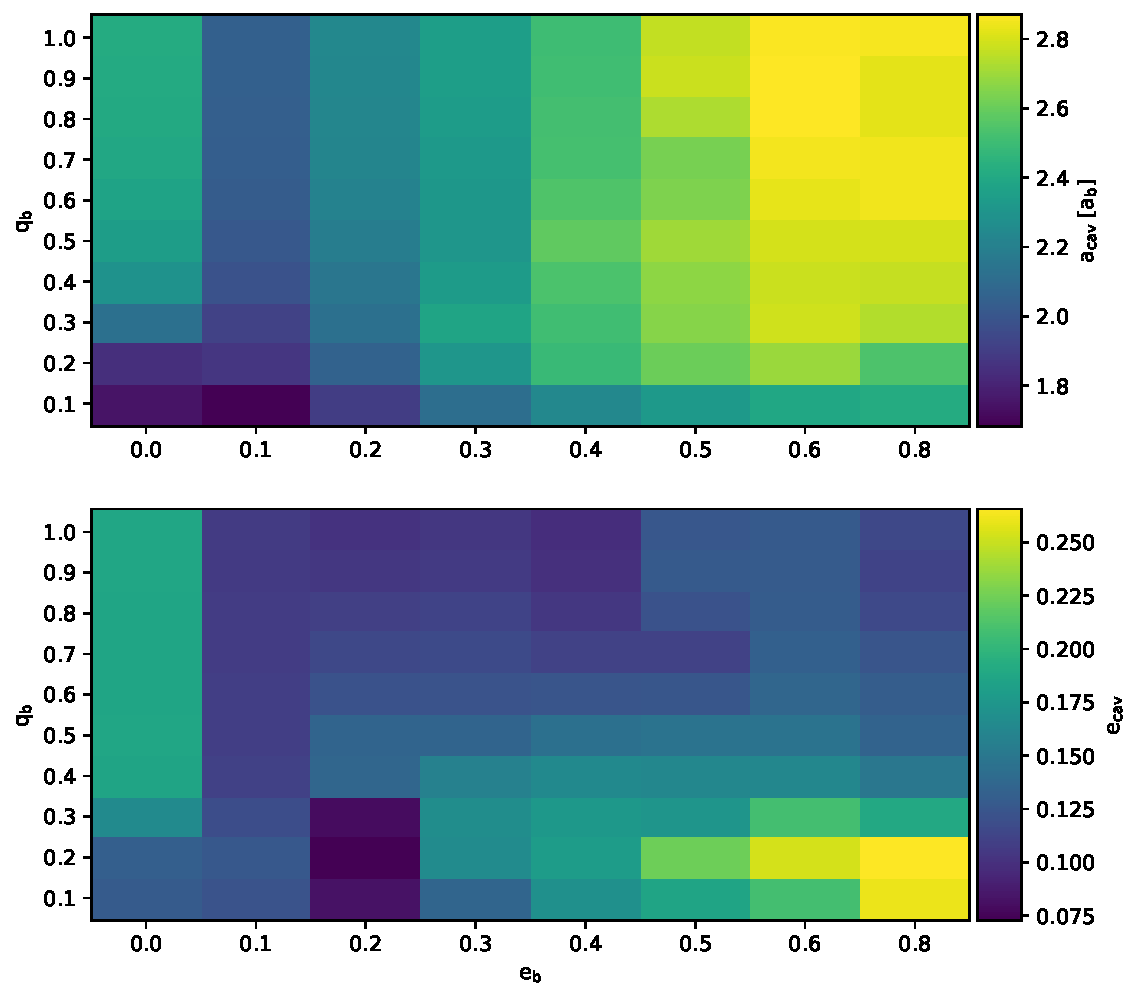
\includegraphics[width=1\columnwidth]{a_e_cavity_heatmap_joint.pdf}
    \caption{Reproduction of Figure 18 from \citet{DeLaurentiis25}, displaying the semi-major axis and eccentricity of the cavities of our simulations with varying binary eccentricity and mass ratio. The cavity is characterized by the $m=1$ Fourier mode of the CBD cavity}
    \label{fig:a_e_cav_heatmap}
\end{figure}

\bibliographystyle{mnras}
\bibliography{main}

% Don't change these lines
\bsp	% typesetting comment
\label{lastpage}


\end{document}